\documentclass{skripsi}

% -------------------------------------------------------------------
% METADATA DOKUMEN SKRIPSI
% -------------------------------------------------------------------
\judulindonesia{Strategi Pemasaran Rumah Makan Nasi Gerilya pada Platform GrabFood untuk Meningkatkan Penjualan Berdasarkan Analisis SWOT}
\judulindonesiacapitalize{Strategi Pemasaran Rumah Makan Nasi Gerilya \\ pada Platform GrabFood untuk Meningkatkan \\ Penjualan Berdasarkan Analisis SWOT}
\judulindonesiacapslock{STRATEGI PEMASARAN RUMAH MAKAN NASI GERILYA \\ PADA PLATFORM GRABFOOD UNTUK MENINGKATKAN \\ PENJUALAN BERDASARKAN ANALISIS SWOT}

\judulinggris{Marketing Strategy of Nasi Gerilya Restaurant on the GrabFood Platform to Increase Sales Based on SWOT Analysis}
\judulinggriscapitalize{Marketing Strategy of Nasi Gerilya Restaurant \\ on the GrabFood Platform to Increase Sales \\ Based on SWOT Analysis}
\judulinggriscapslock{MARKETING STRATEGY OF NASI GERILYA RESTAURANT \\ ON THE GRABFOOD PLATFORM TO INCREASE SALES \\ BASED ON SWOT ANALYSIS}

\author{Marsia Br Pelawi}
\nim{220502068}
\programstudi{Strata 1 Manajemen}
\fakultas{Ekonomi dan Bisnis}
\universitas{Universitas Sumatera Utara}
\tahun{2026}
\kota{Medan}
\tanggalpengesahan{06 Mei 2026}
\labelpenandatangan{Peneliti}
\namapenandatangan{Marsia Br Pelawi}
\logopath{resource/01-brand/logo-usu.png} % Path logo universitas


% Tambahkan .bib file untuk daftar pustaka
\addbibresource{referensi.bib}
\usepackage{pgfplots}
\pgfplotsset{compat=1.18}

\begin{document}

% -------------------------------------------------------------------
% BAGIAN AWAL (FRONTMATTER)
% -------------------------------------------------------------------
\pagenumbering{roman} % Halaman angka romawi kecil (i, ii, iii)
\pagestyle{plain} % Halaman diletakkan di bawah-tengah

\makecover

% DAFTAR ISI
\clearpage
\phantomsection
\addcontentsline{toc}{chapter}{DAFTAR ISI}
\renewcommand{\contentsname}{DAFTAR ISI}
{\singlespacing
\tableofcontents
}

% DAFTAR TABEL
\clearpage
\phantomsection
\addcontentsline{toc}{chapter}{DAFTAR TABEL}
\renewcommand{\listtablename}{DAFTAR TABEL}
\listoftables

% DAFTAR GAMBAR
\clearpage
\phantomsection
\addcontentsline{toc}{chapter}{DAFTAR GAMBAR}
\renewcommand{\listfigurename}{DAFTAR GAMBAR}
\listoffigures

% DAFTAR LAMPIRAN
\clearpage
\phantomsection
\addcontentsline{toc}{chapter}{DAFTAR LAMPIRAN}
\listoflampiran


% -------------------------------------------------------------------
% BAGIAN ISI (MAINMATTER)
% -------------------------------------------------------------------
\clearpage
\pagenumbering{arabic} % Halaman menggunakan angka arab (1, 2, 3)
\pagestyle{skripsi_standard} % Halaman isi selain pembuka bab di kanan atas

\chapter{PENDAHULUAN}

\section{Latar Belakang}
Bisnis kuliner merupakan salah satu sektor usaha yang terus berkembang di Indonesia karena berkaitan langsung dengan kebutuhan konsumsi harian, perubahan gaya hidup masyarakat, serta meningkatnya pemanfaatan kanal digital dalam aktivitas pembelian makanan. Data Badan Pusat Statistik menunjukkan bahwa jumlah usaha penyediaan makanan dan minuman di Indonesia pada 2023 mencapai 4,85 juta usaha, meningkat 21,13\% dibandingkan 2016 yang berjumlah 4,01 juta usaha. Pada tahun yang sama, sektor ini menyerap 9,80 juta tenaga kerja dan menghasilkan nilai penjualan sebesar Rp998,37 triliun, meningkat 48,04\% dibandingkan 2016 \parencite{bps2024pmm}. Perkembangan tersebut berlanjut pada 2024, ketika jumlah usaha penyediaan makanan dan minuman di Indonesia meningkat menjadi 5,28 juta usaha \parencite{bps2025pmm}. Data ini menunjukkan bahwa usaha kuliner bukan hanya memiliki peran ekonomi yang besar, tetapi juga berkembang sebagai ruang usaha yang semakin padat pelaku.

Perkembangan usaha kuliner juga terlihat pada konteks Kota Medan. Sebagai pusat kegiatan ekonomi di Sumatera Utara, Kota Medan memiliki aktivitas konsumsi, perdagangan, dan jasa yang kuat. Dalam data PDRB menurut lapangan usaha, indikator BPS Kota Medan yang paling dekat dengan kegiatan kuliner berada pada kategori penyediaan akomodasi dan makan minum. Pada 2024, kategori ini menjadi lapangan usaha dengan pertumbuhan tertinggi di Kota Medan, yaitu 14,50\%, serta memiliki distribusi sebesar 3,06\% terhadap PDRB Kota Medan \parencite{bpsmedan2025ekonomi}. Kondisi tersebut memperlihatkan bahwa kegiatan makan dan minum menjadi bagian dari dinamika ekonomi perkotaan Medan yang terus bergerak, baik melalui usaha berskala besar maupun usaha kuliner lokal.

Tren perkembangan usaha kuliner nasional dan kategori penyediaan akomodasi dan makan minum di Kota Medan divisualisasikan pada Gambar~\ref{fig:tren-pdb-makan-minum-indonesia} dan Gambar~\ref{fig:tren-pdrb-makan-minum-medan}. Gambar~\ref{fig:tren-pdb-makan-minum-indonesia} menunjukkan bahwa PDB lapangan usaha penyediaan akomodasi dan makan minum atas dasar harga berlaku meningkat dari Rp394,06 triliun pada 2020 menjadi sekitar Rp638,41 triliun pada 2025. Sementara itu, Gambar~\ref{fig:tren-pdrb-makan-minum-medan} menunjukkan bahwa PDRB lapangan usaha penyediaan akomodasi dan makan minum di Kota Medan atas dasar harga berlaku meningkat dari Rp6,62 triliun pada 2020 menjadi Rp10,73 triliun pada 2025. Angka 2025 pada data Kota Medan merupakan angka sangat sementara dari BPS \parencite{bps2025pendapatan,bps2026ekonomiindonesia,bpsmedan2025pdrb,bpsmedan2026pdrb}. Dalam publikasi BPS, kategori ini mencakup penyediaan akomodasi jangka pendek serta penyediaan makanan dan minuman untuk konsumsi segera, sehingga digunakan sebagai indikator resmi yang paling dekat untuk membaca dinamika usaha kuliner dalam struktur PDRB Kota Medan \parencite{bpsmedan2025pdrb,bpsmedan2026pdrb}.

\begin{figure}[!t]
    \centering
    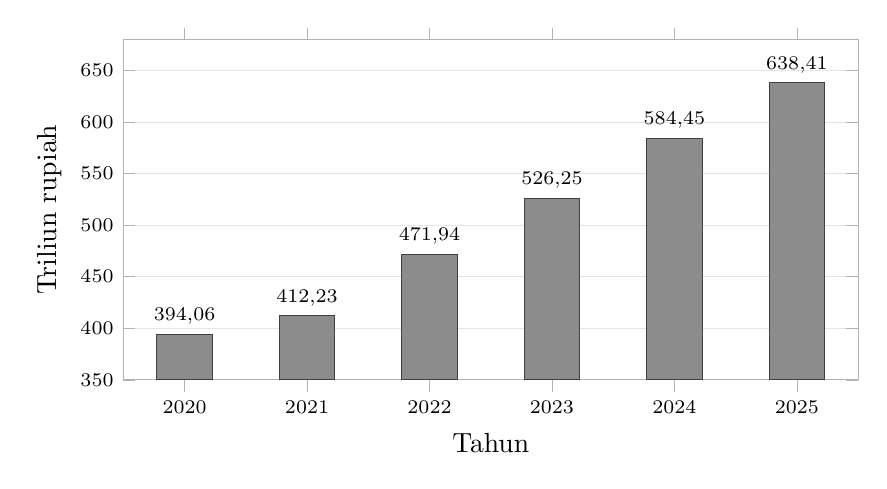
\begin{tikzpicture}
        \begin{axis}[
                width=0.9\textwidth,
                height=5.9cm,
                ybar,
                bar width=20pt,
                ymin=350, ymax=680,
                ylabel={Triliun rupiah},
                xlabel={Tahun},
                symbolic x coords={2020,2021,2022,2023,2024,2025},
                xtick=data,
                ymajorgrids=true,
                grid style={gray!20},
                axis line style={gray!60},
                tick style={gray!60},
                ytick={350,400,450,500,550,600,650},
                yticklabel style={font=\scriptsize},
                x tick label style={font=\scriptsize},
                enlarge x limits=0.10,
                clip=false
            ]
            \addplot[
                fill=black!45,
                draw=black!75
            ] coordinates {
                    (2020,394.06) (2021,412.23) (2022,471.94) (2023,526.25) (2024,584.45) (2025,638.41)
                };
            \node[font=\scriptsize, anchor=south] at (axis cs:2020,394.06) {394,06};
            \node[font=\scriptsize, anchor=south] at (axis cs:2021,412.23) {412,23};
            \node[font=\scriptsize, anchor=south] at (axis cs:2022,471.94) {471,94};
            \node[font=\scriptsize, anchor=south] at (axis cs:2023,526.25) {526,25};
            \node[font=\scriptsize, anchor=south] at (axis cs:2024,584.45) {584,45};
            \node[font=\scriptsize, anchor=south] at (axis cs:2025,638.41) {638,41};
        \end{axis}
    \end{tikzpicture}
    \figuresource[0.9\textwidth]{Diolah peneliti dari BPS \parencite{bps2025pendapatan,bps2026ekonomiindonesia}.}
    \caption{Tren PDB lapangan usaha penyediaan akomodasi dan makan minum di Indonesia atas dasar harga berlaku}
    \label{fig:tren-pdb-makan-minum-indonesia}
\end{figure}

\begin{figure}[!t]
    \centering
    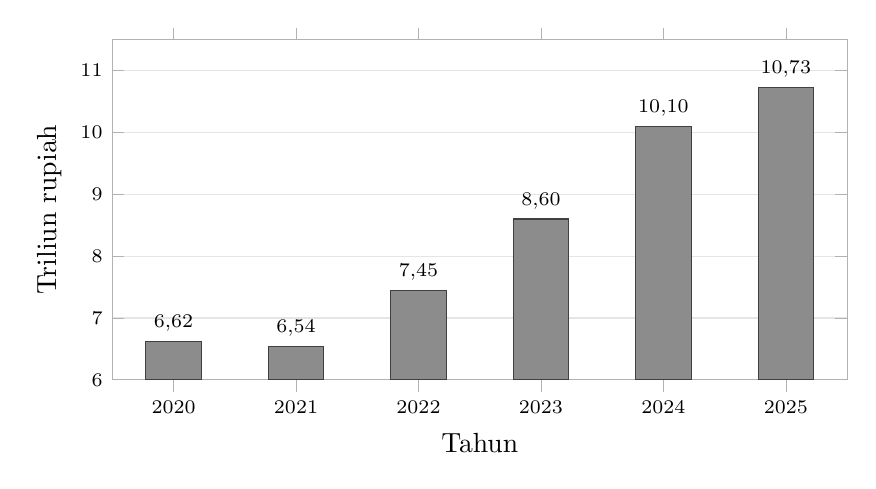
\begin{tikzpicture}
        \begin{axis}[
                width=0.9\textwidth,
                height=5.9cm,
                ybar,
                bar width=20pt,
                ymin=6, ymax=11.5,
                ylabel={Triliun rupiah},
                xlabel={Tahun},
                symbolic x coords={2020,2021,2022,2023,2024,2025},
                xtick=data,
                ymajorgrids=true,
                grid style={gray!20},
                axis line style={gray!60},
                tick style={gray!60},
                ytick={6,7,8,9,10,11},
                yticklabel style={font=\scriptsize},
                x tick label style={font=\scriptsize},
                enlarge x limits=0.10,
                clip=false
            ]
            \addplot[
                fill=black!45,
                draw=black!75
            ] coordinates {
                    (2020,6.62) (2021,6.54) (2022,7.45) (2023,8.60) (2024,10.10) (2025,10.73)
                };
            \node[font=\scriptsize, anchor=south] at (axis cs:2020,6.62) {6,62};
            \node[font=\scriptsize, anchor=south] at (axis cs:2021,6.54) {6,54};
            \node[font=\scriptsize, anchor=south] at (axis cs:2022,7.45) {7,45};
            \node[font=\scriptsize, anchor=south] at (axis cs:2023,8.60) {8,60};
            \node[font=\scriptsize, anchor=south] at (axis cs:2024,10.10) {10,10};
            \node[font=\scriptsize, anchor=south] at (axis cs:2025,10.73) {10,73};
        \end{axis}
    \end{tikzpicture}
    \figuresource[0.9\textwidth]{Diolah peneliti dari BPS Kota Medan \parencite{bpsmedan2025pdrb,bpsmedan2026pdrb}.}
    \caption{Tren PDRB lapangan usaha penyediaan akomodasi dan makan minum di Kota Medan atas dasar harga berlaku}
    \label{fig:tren-pdrb-makan-minum-medan}
\end{figure}

Pertumbuhan jumlah usaha kuliner menyebabkan tingkat persaingan semakin ketat. Pelaku usaha tidak hanya bersaing dari sisi rasa, tetapi juga dari variasi menu, harga, kemasan, lokasi, kecepatan layanan, promosi, reputasi, dan kemudahan akses pembelian. Dalam kondisi pasar yang padat, usaha kuliner membutuhkan strategi pemasaran yang efektif agar mampu menarik pelanggan baru, mempertahankan pelanggan lama, dan menjaga daya saing terhadap kompetitor. Pemasaran dalam konteks ini dipahami sebagai proses menciptakan, mengomunikasikan, menyampaikan, dan mempertukarkan nilai kepada konsumen \parencite{kotler2021marketingmanagement}. Oleh karena itu, strategi pemasaran perlu disusun berdasarkan pemahaman terhadap kebutuhan pasar, karakter konsumen, kekuatan usaha, serta tekanan persaingan yang dihadapi.

Pemasaran usaha kuliner dapat dilakukan melalui saluran offline dan online. Pemasaran offline umumnya dilakukan melalui lokasi fisik, papan nama, rekomendasi dari mulut ke mulut, pelayanan langsung, kerja sama komunitas, dan promosi di sekitar area usaha. Sementara itu, pemasaran online dilakukan melalui media sosial, katalog digital, mesin pencari, aplikasi pesan, marketplace, serta platform pesan antar makanan. Perkembangan pemasaran digital menjadi penting karena konsumen kini dapat menemukan, membandingkan, memesan, dan menilai produk kuliner melalui perangkat digital \parencite{chaffey2022digitalmarketing,regina2025kuliner}. Bagi UMKM kuliner, penggunaan kanal digital dapat memperluas jangkauan pasar, meningkatkan visibilitas, dan mempercepat transaksi ketika dikelola secara konsisten \parencite{regina2025kuliner,mamuriyah2021gadihminang,roslam2021markisaaurora,suharjo2020bogorsnacks}.

Salah satu bentuk pemasaran online yang banyak digunakan pelaku usaha kuliner adalah platform marketplace atau \textit{online food delivery} seperti ShopeeFood, GoFood, dan GrabFood. Platform tersebut tidak hanya berfungsi sebagai media pemesanan, tetapi juga menjadi etalase digital yang menampilkan nama usaha, foto menu, harga, promo, rating, ulasan pelanggan, dan estimasi layanan. Kajian terdahulu menunjukkan bahwa pemanfaatan platform digital dapat membantu UMKM memperluas jangkauan pasar dan meningkatkan penjualan ketika fitur platform, promosi, tampilan produk, serta komunikasi dengan pelanggan dikelola secara konsisten \parencite{regina2025kuliner,sophia2025rendanggadih,suharjo2020bogorsnacks}. Hal ini menunjukkan bahwa platform seperti GrabFood telah menjadi ruang pemasaran dan persaingan yang penting bagi usaha kuliner.

Rumah Makan Nasi Gerilya merupakan usaha nasi Padang di Kota Medan yang memanfaatkan kanal online dalam aktivitas penjualannya. Berdasarkan wawancara awal dengan pemilik, Nasi Gerilya menggunakan GrabFood, GoFood, dan ShopeeFood sebagai kanal penjualan online, tetapi GrabFood menjadi platform utama karena dinilai paling sesuai dengan target pasar usaha. Pemilik juga menyampaikan bahwa GrabFood berkontribusi lebih dari 50\% terhadap \textit{revenue} usaha, sehingga platform ini tidak hanya berperan sebagai saluran tambahan, tetapi sebagai salah satu kanal penjualan utama. Hasil observasi toko pada GrabFood menunjukkan bahwa Nasi Gerilya memiliki rating 4,7/5,0, 4.187 ulasan, rentang harga Rp11.000--Rp72.000, promo platform aktif, serta menu teratas seperti rendang sapi, ayam goreng, ayam bakar, dan nasi bakar kikil tunjang. Keempat menu teratas tersebut menunjukkan variasi harga utama yang ditawarkan Nasi Gerilya pada GrabFood sebagaimana disajikan pada Tabel~\ref{tab:harga-menu-teratas-gerilya}.

\begin{table}[!t]
    \centering
    \caption{Harga Menu Teratas Rumah Makan Nasi Gerilya pada GrabFood}
    \label{tab:harga-menu-teratas-gerilya}
    \small
    \renewcommand{\arraystretch}{1.08}
    \begin{tabularx}{0.82\textwidth}{|X|>{\raggedleft\arraybackslash}p{3cm}|}
        \toprule
        \textbf{Menu Teratas}    & \textbf{Harga} \\ \hline
        \midrule
        Nasi Padang Rendang Sapi & Rp56.000       \\ \hline
        Nasi Padang Ayam Goreng  & Rp45.000       \\ \hline
        Nasi Padang Ayam Bakar   & Rp45.000       \\ \hline
        Nasi Bakar Kikil Tunjang & Rp68.000       \\ \hline
        \bottomrule
    \end{tabularx}
    \tablesource[0.82\textwidth]{Observasi platform GrabFood pada 04 April 2026; diolah peneliti (2026).}
\end{table}

Menu selebihnya disajikan secara lebih lengkap pada Lampiran Tabel~\ref{tab:survei_harga_nasi_gerilya_grabfood}. Data awal mengenai observasi GrabFood, wawancara awal pemilik, dan dokumentasi kinerja usaha disajikan lebih lengkap pada Lampiran~\ref{app:observasi-grabfood}, Lampiran~\ref{app:wawancara-awal-pemilik}, dan Lampiran~\ref{app:dokumentasi-indeks-kinerja}. Visual pendukung pada Gambar~\ref{fig:tren-penjualan-bungkus-gerilya} menunjukkan bahwa jumlah penjualan Nasi Gerilya meningkat dari 6.702 bungkus pada Desember 2024 menjadi 16.590 bungkus pada Maret 2025, tetapi kemudian menurun bertahap menjadi 12.900 bungkus pada November 2025. Gambar~\ref{fig:komposisi-pelanggan-gerilya} juga menunjukkan bahwa pelanggan baru meningkat dari 45\% menjadi 55\%, sedangkan \textit{repeat order} menurun dari 43\% menjadi 38\%. Kondisi tersebut menunjukkan bahwa eksposur digital dan kontribusi GrabFood yang besar belum otomatis menjamin stabilitas penjualan dan loyalitas pelanggan.

\begin{figure}[!t]
    \centering
    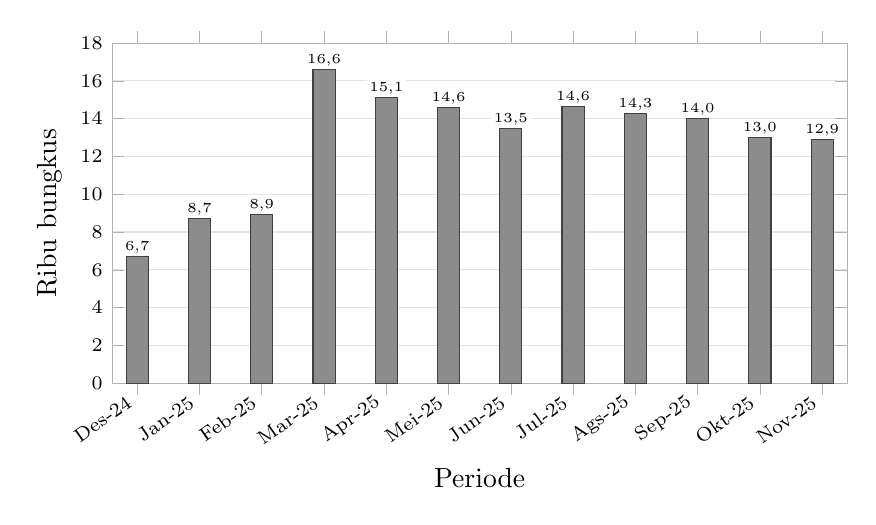
\begin{tikzpicture}
        \begin{axis}[
                width=0.9\textwidth,
                height=5.9cm,
                ybar,
                bar width=8pt,
                xmin=-0.4, xmax=11.4,
                ymin=0, ymax=18,
                ylabel={Ribu bungkus},
                xlabel={Periode},
                ymajorgrids=true,
                grid style={gray!20},
                axis line style={gray!60},
                tick style={gray!60},
                xtick=data,
                xticklabels={Des-24,Jan-25,Feb-25,Mar-25,Apr-25,Mei-25,Jun-25,Jul-25,Ags-25,Sep-25,Okt-25,Nov-25},
                x tick label style={rotate=35, anchor=east, font=\scriptsize},
                ytick={0,2,4,6,8,10,12,14,16,18},
                yticklabel style={font=\scriptsize},
                clip=false
            ]
            \addplot[
                fill=black!45,
                draw=black!75
            ] coordinates {
                    (0,6.702) (1,8.740) (2,8.911) (3,16.590) (4,15.129) (5,14.580)
                    (6,13.467) (7,14.633) (8,14.259) (9,14.034) (10,13.009) (11,12.900)
                };
            \node[font=\tiny, fill=white, inner sep=1pt, anchor=south] at (axis cs:0,6.702) {6,7};
            \node[font=\tiny, fill=white, inner sep=1pt, anchor=south] at (axis cs:1,8.740) {8,7};
            \node[font=\tiny, fill=white, inner sep=1pt, anchor=south] at (axis cs:2,8.911) {8,9};
            \node[font=\tiny, fill=white, inner sep=1pt, anchor=south] at (axis cs:3,16.590) {16,6};
            \node[font=\tiny, fill=white, inner sep=1pt, anchor=south] at (axis cs:4,15.129) {15,1};
            \node[font=\tiny, fill=white, inner sep=1pt, anchor=south] at (axis cs:5,14.580) {14,6};
            \node[font=\tiny, fill=white, inner sep=1pt, anchor=south] at (axis cs:6,13.467) {13,5};
            \node[font=\tiny, fill=white, inner sep=1pt, anchor=south] at (axis cs:7,14.633) {14,6};
            \node[font=\tiny, fill=white, inner sep=1pt, anchor=south] at (axis cs:8,14.259) {14,3};
            \node[font=\tiny, fill=white, inner sep=1pt, anchor=south] at (axis cs:9,14.034) {14,0};
            \node[font=\tiny, fill=white, inner sep=1pt, anchor=south] at (axis cs:10,13.009) {13,0};
            \node[font=\tiny, fill=white, inner sep=1pt, anchor=south] at (axis cs:11,12.900) {12,9};
        \end{axis}
    \end{tikzpicture}
    \figuresource[0.9\textwidth]{Diolah peneliti dari dokumentasi grafik penjualan bulanan Nasi Gerilya.}
    \caption{Tren jumlah penjualan bulanan Nasi Gerilya dalam satuan bungkus}
    \label{fig:tren-penjualan-bungkus-gerilya}
\end{figure}

\begin{figure}[!t]
    \centering
    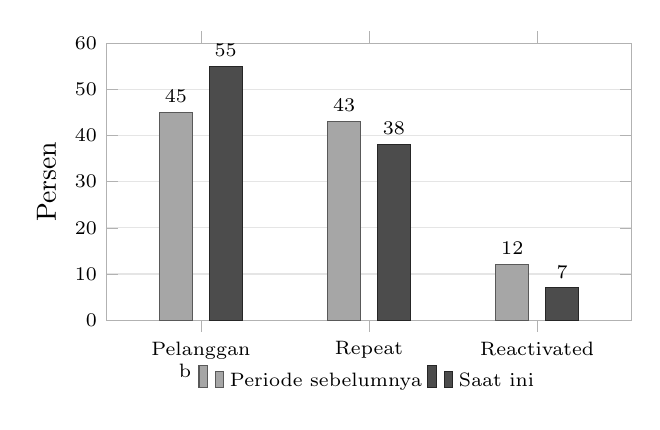
\begin{tikzpicture}
        \begin{axis}[
                width=0.68\textwidth,
                height=5.1cm,
                ybar=6pt,
                bar width=12pt,
                ymin=0, ymax=60,
                ylabel={Persen},
                ymajorgrids=true,
                grid style={gray!20},
                axis line style={gray!60},
                tick style={gray!60},
                symbolic x coords={Baru,Repeat,Reactivated},
                xtick=data,
                xticklabels={Pelanggan\\baru,Repeat\\order,Reactivated},
                x tick label style={font=\scriptsize, align=center},
                ytick={0,10,20,30,40,50,60},
                yticklabel style={font=\scriptsize},
                nodes near coords,
                every node near coord/.append style={font=\scriptsize},
                enlarge x limits=0.28,
                legend style={
                        font=\scriptsize,
                        draw=none,
                        at={(0.5,-0.14)},
                        anchor=north,
                        legend columns=2
                    }
            ]
            \addplot[fill=black!35, draw=black!65] coordinates {(Baru,45) (Repeat,43) (Reactivated,12)};
            \addplot[fill=black!70, draw=black!85] coordinates {(Baru,55) (Repeat,38) (Reactivated,7)};
            \legend{Periode sebelumnya,Saat ini}
        \end{axis}
    \end{tikzpicture}
    \figuresource[0.68\textwidth]{Diolah peneliti dari wawancara awal dengan pemilik usaha.}
    \caption{Perubahan komposisi pelanggan Nasi Gerilya berdasarkan wawancara awal pemilik usaha}
    \label{fig:komposisi-pelanggan-gerilya}
\end{figure}
Dalam kondisi tersebut, bauran pemasaran atau \textit{marketing mix} menjadi konsep yang relevan untuk membaca strategi pemasaran Nasi Gerilya. Konsep 4P menempatkan \textit{product}, \textit{price}, \textit{place}, dan \textit{promotion} sebagai perangkat utama dalam mengelola penawaran pasar \parencite{kotler2023principlesmarketing}. Pada bisnis jasa dan kuliner, bauran tersebut dapat diperluas menjadi 7P dengan menambahkan \textit{people}, \textit{process}, dan \textit{physical evidence} karena pengalaman pelanggan juga dipengaruhi oleh pelaksana layanan, proses pemenuhan pesanan, serta bukti kualitas yang terlihat oleh konsumen \parencite{wirtz2024servicesmarketing}. Dalam konteks Nasi Gerilya pada GrabFood, unsur produk terlihat dari variasi menu dan konsistensi rasa; harga terlihat dari rentang harga, ongkos kirim, dan promo; tempat terlihat dari penggunaan GrabFood sebagai kanal distribusi online; promosi terlihat dari voucher, promo platform, media sosial, dan KOL; \textit{people} terlihat dari kesiapan admin, karyawan, dan juru masak; \textit{process} terlihat dari kecepatan layanan, pengelolaan menu habis, dan ketepatan pesanan; sedangkan \textit{physical evidence} terlihat dari foto produk, kemasan, rating, dan ulasan pelanggan.

Review pelanggan menjadi bagian penting dalam evaluasi strategi pemasaran karena platform \textit{online food delivery} membuat pengalaman pelanggan terekam secara terbuka melalui rating, komentar, keluhan, dan rekomendasi. Penelitian terdahulu menunjukkan bahwa harga, promosi, tampilan produk, kualitas layanan, ulasan, dan peringkat pada platform digital dapat memengaruhi keputusan pembelian serta performa penjualan usaha kuliner \parencite{sophia2025rendanggadih,ruhiyat2023minatbeli,khairani2022buahsayur,suharjo2020bogorsnacks}. Pada Nasi Gerilya, review pelanggan memuat komentar positif mengenai rasa enak, bumbu dan rempah yang kuat, porsi besar, bahan segar, kemasan rapi, variasi menu, serta harga yang dinilai terjangkau. Namun, review tersebut juga memuat keluhan mengenai rasa yang dianggap berubah, pesanan tidak lengkap, menu tidak tersedia, lauk utama yang dinilai kurang besar atau kurang segar, nasi yang kadang keras, proporsi nasi dan lauk yang kurang seimbang, serta suhu makanan yang tidak selalu konsisten. Oleh karena itu, review pelanggan, komentar, keluhan, dan permasalahan layanan menjadi dasar penting untuk mengevaluasi serta meningkatkan strategi pemasaran Nasi Gerilya pada GrabFood.

\section{Rumusan Masalah}
Berdasarkan latar belakang di atas, maka rumusan masalah dalam penelitian ini adalah:
\begin{enumerate}
    \item Bagaimana faktor internal Rumah Makan Nasi Gerilya pada platform GrabFood yang mencakup kekuatan dan kelemahan usaha?
    \item Bagaimana faktor eksternal Rumah Makan Nasi Gerilya pada platform GrabFood yang mencakup peluang dan ancaman usaha?
    \item Bagaimana strategi pemasaran Rumah Makan Nasi Gerilya pada platform GrabFood berdasarkan analisis matriks SWOT?
\end{enumerate}

\section{Tujuan Penelitian}
Tujuan yang ingin dicapai dalam penelitian ini adalah sebagai berikut:
\begin{enumerate}
    \item Untuk mengidentifikasi faktor internal Rumah Makan Nasi Gerilya pada platform GrabFood yang mencakup kekuatan dan kelemahan usaha.
    \item Untuk mengidentifikasi faktor eksternal Rumah Makan Nasi Gerilya pada platform GrabFood yang mencakup peluang dan ancaman usaha.
    \item Untuk merumuskan strategi pemasaran Rumah Makan Nasi Gerilya pada platform GrabFood berdasarkan analisis matriks SWOT.
\end{enumerate}

\section{Manfaat Penelitian}
Penelitian ini diharapkan dapat bermanfaat secara teoretis dan praktis:
\subsection{Manfaat Teoretis}
Penelitian ini diharapkan dapat berkontribusi dalam pengembangan ilmu manajemen pemasaran, khususnya yang berkaitan dengan strategi pemasaran usaha kuliner pada platform \textit{online food delivery}, terutama GrabFood. Selain itu, penelitian ini juga diharapkan dapat memperkaya kajian mengenai penerapan analisis SWOT dalam mengidentifikasi faktor internal dan faktor eksternal usaha sebagai dasar perumusan strategi pemasaran. Hasil penelitian ini selanjutnya diharapkan dapat menjadi bahan referensi bagi peneliti lain yang ingin mengkaji topik serupa, terutama pada konteks UMKM kuliner yang memanfaatkan platform digital sebagai saluran pemasaran.
\subsection{Manfaat Praktis}
Secara praktis, penelitian ini diharapkan dapat memberikan manfaat bagi beberapa pihak sebagai berikut:
\subsubsection{Bagi Rumah Makan Nasi Gerilya}
\noindent Penelitian ini diharapkan dapat menjadi bahan masukan dan evaluasi dalam mengidentifikasi kekuatan, kelemahan, peluang, dan ancaman usaha pada platform GrabFood. Dengan demikian, hasil penelitian ini dapat digunakan sebagai dasar dalam merumuskan strategi pemasaran yang lebih tepat untuk mempertahankan daya saing dan meningkatkan kinerja usaha.
\subsubsection{Bagi Pelaku Usaha Kuliner}
\noindent Penelitian ini diharapkan dapat menjadi gambaran dan bahan pertimbangan bagi pelaku usaha kuliner lainnya mengenai pentingnya analisis kondisi internal dan eksternal usaha dalam menyusun strategi pemasaran pada platform \textit{online food delivery}.
\subsubsection{Bagi Akademisi}
\noindent Penelitian ini diharapkan dapat menjadi tambahan acuan dan referensi ilmiah, khususnya yang berkaitan dengan strategi pemasaran kuliner berbasis platform, strategi pemasaran UMKM, dan penerapan analisis SWOT pada sektor kuliner.

\chapter{TINJAUAN PUSTAKA}

\section{Landasan Teoritis}
\subsection{Pemasaran}
Pemasaran merupakan konsep dasar yang perlu dijelaskan terlebih dahulu karena penelitian ini membahas cara Rumah Makan Nasi Gerilya menyusun penawaran dan menjangkau konsumen melalui GrabFood. Pemasaran tidak hanya berarti kegiatan menjual atau mempromosikan produk, tetapi mencakup proses menciptakan, mengomunikasikan, menyampaikan, dan mempertukarkan nilai kepada pelanggan secara menguntungkan \parencite{kotler2021marketingmanagement,kotler2023principlesmarketing}. Dalam pandangan pemasaran modern, nilai pelanggan terbentuk ketika kebutuhan konsumen, kemampuan usaha, dan penawaran pasar bertemu dalam bentuk produk, harga, akses pembelian, komunikasi, serta pengalaman layanan yang dianggap relevan oleh konsumen \parencite{kotler2023principlesmarketing,wirtz2024servicesmarketing}. Karena itu, pemasaran menjadi landasan untuk memahami mengapa sebuah usaha kuliner tidak cukup hanya memiliki produk yang baik, tetapi juga perlu mengelola cara produk tersebut dipersepsikan, ditemukan, dipilih, dibeli, dan dinilai oleh konsumen.

Pada usaha kuliner, pemasaran berperan sebagai penghubung antara kemampuan internal usaha dengan kebutuhan pasar yang terus berubah. Konsumen makanan tidak hanya menilai cita rasa, tetapi juga variasi menu, keterjangkauan harga, kemudahan akses, kecepatan layanan, tampilan produk, reputasi, serta konsistensi pengalaman pembelian \parencite{regina2025kuliner,sophia2025rendanggadih,wirtz2024servicesmarketing}. Ketika pembelian dilakukan melalui platform digital, ruang pemasaran semakin meluas karena konsumen mengambil keputusan berdasarkan informasi yang tersaji di aplikasi, seperti nama menu, foto produk, deskripsi, harga, promo, rating, dan ulasan \parencite{hidayah2021digitalplatforms,putri2024cikarang,elverda2025ofdindonesia}. Dengan demikian, pemasaran dalam penelitian ini menjadi pijakan awal untuk membaca aktivitas Nasi Gerilya sebagai upaya menyusun nilai produk dan pengalaman pembelian yang sesuai dengan karakter pasar digital.

\subsection{Strategi Pemasaran}
Strategi pemasaran merupakan kelanjutan dari konsep pemasaran karena strategi menjelaskan arah dan cara usaha mengelola nilai yang ditawarkan kepada pasar sasaran. Dalam pemasaran modern, strategi tidak hanya dipahami sebagai kegiatan promosi, tetapi sebagai keputusan terpadu mengenai siapa yang dilayani, nilai apa yang ditawarkan, dan bagaimana nilai tersebut disampaikan secara lebih unggul daripada pesaing \parencite{kotler2021marketingmanagement,kotler2023principlesmarketing}. Pemahaman ini sejalan dengan pandangan manajemen strategis yang menempatkan strategi sebagai proses penyesuaian antara tujuan organisasi, kemampuan internal, dan tekanan lingkungan eksternal \parencite{david2023strategicmanagement}. Dengan demikian, strategi pemasaran perlu dibaca sebagai jembatan antara tujuan usaha dan kondisi pasar yang dihadapi, bukan sebagai kegiatan yang berdiri sendiri.

Pada usaha kuliner, strategi pemasaran semakin penting karena persaingan tidak hanya berlangsung pada kualitas rasa, tetapi juga pada variasi menu, harga, kemasan, promosi, akses pemesanan, dan pengalaman layanan yang melekat pada proses pembelian \parencite{regina2025kuliner,sophia2025rendanggadih}. Perubahan menuju pemasaran digital membuat keputusan strategis menjadi lebih kompleks karena usaha perlu mengelola tampilan produk, informasi menu, promosi, dan kanal transaksi secara bersamaan \parencite{chaffey2022digitalmarketing,hidayah2021digitalplatforms}. Dalam konteks UMKM kuliner, penelitian sebelumnya menunjukkan bahwa penguatan strategi digital dapat membantu meningkatkan visibilitas, memperluas jangkauan pasar, dan memperbaiki kinerja usaha ketika didukung oleh kesiapan organisasi serta pemilihan kanal yang tepat \parencite{putro2025digitaltransformation,regina2025kuliner}. Oleh karena itu, strategi pemasaran pada Rumah Makan Nasi Gerilya perlu dipahami sebagai rangkaian keputusan yang menghubungkan kekuatan produk, pengelolaan platform GrabFood, dan respons terhadap persaingan pasar.

Strategi tersebut harus mampu menerjemahkan pemahaman tentang konsumen menjadi keputusan yang lebih operasional, mulai dari penentuan pasar sasaran, posisi usaha, susunan menu, harga, promosi, saluran pemasaran, hingga cara usaha merespons peluang dan ancaman di dalam platform \parencite{kotler2023principlesmarketing,chaffey2022digitalmarketing,david2023strategicmanagement}. Karena fokus penelitian ini adalah perumusan strategi, konsep strategi pemasaran menjadi dasar untuk menempatkan STP, bauran pemasaran, pemasaran digital, saluran OFDA, analisis lingkungan, dan SWOT sebagai bagian yang saling melengkapi.

\subsection{STP dan Bauran Pemasaran}
Segmentasi, \textit{targeting}, dan \textit{positioning} (STP) melengkapi strategi pemasaran karena membantu usaha menentukan kelompok pasar yang ingin dilayani dan citra yang ingin dibangun di benak konsumen \parencite{kotler2021marketingmanagement,kotler2023principlesmarketing}. Segmentasi diperlukan karena pasar kuliner tidak homogen; konsumen dapat berbeda dalam daya beli, waktu pembelian, preferensi menu, sensitivitas harga, dan respons terhadap promosi \parencite{suharjo2020bogorsnacks,ruhiyat2023minatbeli}. Setelah segmen dipahami, usaha perlu memilih segmen yang paling sesuai dengan kapasitas dan tujuan usahanya, lalu membangun \textit{positioning} yang membedakan penawarannya dari pesaing \parencite{kotler2023principlesmarketing,sophia2025rendanggadih}. Pada konteks Nasi Gerilya, STP menjadi penting karena strategi pemasaran di GrabFood perlu menjelaskan pasar sasaran, posisi harga, identitas rasa, dan alasan konsumen memilih usaha tersebut dibanding \textit{merchant} sejenis.

Bauran pemasaran menerjemahkan STP menjadi tindakan pemasaran yang lebih operasional. Konsep 4P menempatkan \textit{product}, \textit{price}, \textit{place}, dan \textit{promotion} sebagai perangkat utama untuk mengelola penawaran pasar \parencite{kotler2021marketingmanagement,kotler2023principlesmarketing}. Dalam usaha kuliner digital, produk tidak hanya berupa makanan, tetapi juga variasi menu, kemasan, foto, dan kejelasan deskripsi; harga tidak hanya berupa nominal menu, tetapi juga potongan harga, ongkos kirim, dan paket promosi; tempat tidak hanya berarti lokasi fisik, tetapi juga kanal distribusi digital; sedangkan promosi mencakup voucher, kampanye platform, dan komunikasi visual \parencite{chaffey2022digitalmarketing,hidayah2021digitalplatforms,putri2024cikarang}. Penelitian tentang strategi pemasaran kuliner berbasis platform juga menunjukkan bahwa penerapan STP dan bauran pemasaran dapat membantu usaha mengarahkan penjualan ketika fitur platform dimanfaatkan secara konsisten \parencite{sophia2025rendanggadih,firdaus2022bangkupawon}.

Pada bisnis jasa dan kuliner, bauran pemasaran sering diperluas menjadi 7P dengan menambahkan \textit{people}, \textit{process}, dan \textit{physical evidence}, karena keberhasilan pemasaran tidak hanya ditentukan oleh penawaran inti, tetapi juga oleh pelaksana layanan, proses pemenuhan pesanan, dan bukti yang memperkuat persepsi kualitas \parencite{wirtz2024servicesmarketing}. Dalam konteks OFDA, unsur tersebut terlihat dari kesiapan admin dan karyawan, kecepatan konfirmasi, akurasi pesanan, pengelolaan menu habis, tampilan etalase digital, foto produk, kemasan, rating, dan ulasan \parencite{hidayah2021digitalplatforms,putri2024cikarang,elverda2025ofdindonesia}. Dengan demikian, STP dan bauran pemasaran saling melengkapi: STP membantu menentukan arah pasar dan posisi usaha, sedangkan bauran pemasaran membantu menilai apakah keputusan produk, harga, distribusi, promosi, proses, pelaksana layanan, dan bukti digital sudah mendukung posisi tersebut.

\subsection{Pemasaran Digital}
Pemasaran digital memperluas pembahasan strategi pemasaran karena teknologi digital mengubah cara usaha menciptakan, mengomunikasikan, dan menyampaikan nilai kepada pasar \parencite{chaffey2022digitalmarketing}. Berbeda dari pemasaran konvensional yang sering bergantung pada komunikasi satu arah, pemasaran digital memungkinkan interaksi, pengukuran respons, dan penyesuaian pesan secara lebih cepat melalui data kunjungan, klik, ulasan, transaksi, dan keterlibatan konsumen \parencite{chaffey2022digitalmarketing,purnomo2023conversion}. Dalam konteks usaha kuliner, pemasaran digital tidak hanya berarti mengunggah konten promosi, tetapi juga mengelola katalog menu, foto produk, deskripsi, promosi, kanal pemesanan, dan reputasi digital \parencite{regina2025kuliner,hidayah2021digitalplatforms}. Dengan demikian, pemasaran digital menjadi bagian dari strategi bisnis yang menghubungkan aktivitas promosi, distribusi, transaksi, dan evaluasi pasar.

Pemasaran digital relevan bagi UMKM kuliner karena usaha kecil sering menghadapi keterbatasan lokasi, modal promosi, dan jangkauan pelanggan, sedangkan platform digital membuka peluang untuk memperluas pasar dengan biaya yang relatif lebih fleksibel \parencite{fatmawatie2022turnover,regina2025kuliner}. Penelitian \textcite{putro2025digitaltransformation} menunjukkan bahwa transformasi digital berpengaruh terhadap kinerja UMKM kuliner melalui dukungan teknologi, organisasi, dan lingkungan. Kajian lain menunjukkan bahwa penggunaan media sosial, katalog daring, \textit{e-commerce}, dan aplikasi pesan antar dapat meningkatkan visibilitas, penjualan, dan keterhubungan usaha dengan konsumen ketika dikelola secara konsisten \parencite{hidayah2021digitalplatforms,indriyani2025gudangbaju,pratama2024sambelmoji}. Oleh karena itu, pemasaran digital dalam penelitian ini diposisikan sebagai konteks strategis yang membantu membaca bagaimana Nasi Gerilya memanfaatkan GrabFood sebagai kanal pemasaran, bukan sekadar sebagai aplikasi pemesanan.

\subsection{Saluran Pemasaran (OFDA)}
\textit{Online food delivery application} (OFDA) merupakan saluran digital yang mempertemukan usaha makanan dengan konsumen melalui sistem yang mengintegrasikan informasi produk, pemesanan, pembayaran, promosi, dan pengantaran \parencite{zaheer2024ofda,elverda2025ofdindonesia}. Dalam kajian strategi pemasaran, OFDA tidak hanya dipahami sebagai alat distribusi, tetapi juga sebagai etalase digital, ruang promosi, sumber reputasi, dan arena persaingan antar \textit{merchant} \parencite{chaffey2022digitalmarketing,putri2024cikarang}. Karakteristik ini membuat keputusan strategi pada platform seperti GrabFood perlu memperhatikan keterpaduan antara menu, harga, foto, deskripsi, promo, ketersediaan toko, rating, dan posisi terhadap pesaing \parencite{hidayah2021digitalplatforms,firdaus2022bangkupawon}.

Peran OFDA dalam usaha kuliner berkaitan langsung dengan bauran pemasaran karena produk ditampilkan melalui nama menu dan visual, harga ditampilkan bersama potongan dan ongkos kirim, distribusi dilakukan melalui jaringan pengantaran, sedangkan promosi dijalankan melalui voucher, kampanye platform, dan paket bundling \parencite{putri2024cikarang,sophia2025rendanggadih}. Penelitian tentang pemanfaatan GrabFood dan GoFood menunjukkan bahwa platform pesan antar dapat membantu UMKM memperluas jangkauan pasar dan meningkatkan penjualan, tetapi manfaat tersebut tetap bergantung pada kemampuan usaha mengelola fitur platform secara tepat \parencite{firdaus2022bangkupawon,putri2024cikarang}. Dengan demikian, OFDA dalam penelitian ini menjadi konteks strategis untuk membaca bagaimana Nasi Gerilya mengelola saluran GrabFood dan bagaimana dinamika platform tersebut memunculkan peluang maupun ancaman bagi strategi pemasaran.

\subsection{Analisis Lingkungan}
Analisis lingkungan diperlukan karena strategi pemasaran harus disusun berdasarkan kondisi nyata usaha dan dinamika pasar yang dihadapi. Dalam manajemen strategis, lingkungan internal menggambarkan sumber daya dan kemampuan yang berada dalam kendali usaha, sedangkan lingkungan eksternal menggambarkan kondisi pasar, pesaing, teknologi, kebijakan, dan perubahan perilaku konsumen yang memengaruhi ruang gerak usaha \parencite{david2023strategicmanagement,kotler2023principlesmarketing}. Dalam kerangka SWOT, faktor internal menjadi dasar untuk menentukan kekuatan dan kelemahan, sedangkan faktor eksternal menjadi dasar untuk menentukan peluang dan ancaman \parencite{gurel2017swot,helms2010swotreview}. Dengan demikian, analisis lingkungan membantu penelitian ini menghindari perumusan strategi yang hanya bertumpu pada keinginan usaha, karena strategi perlu disesuaikan dengan kapasitas internal dan tekanan eksternal.

\subsubsection{Lingkungan Internal}
Lingkungan internal pada usaha kuliner dapat dilihat melalui beberapa bidang, seperti sumber daya manusia, keuangan, produksi, operasional, pemasaran, dan teknologi. Aspek sumber daya manusia berkaitan dengan jumlah karyawan, pembagian tugas, kemampuan mengelola pesanan, kecepatan pelayanan, dan kedisiplinan dalam menjaga standar kerja \parencite{wirtz2024servicesmarketing,david2023strategicmanagement}. Aspek keuangan berkaitan dengan kemampuan usaha mengatur harga, biaya bahan baku, biaya promosi, potongan platform, dan margin penjualan agar strategi promosi tidak menurunkan keberlanjutan usaha \parencite{kotler2023principlesmarketing,david2023strategicmanagement}. Aspek produksi dan operasional mencakup konsistensi rasa, kualitas bahan, variasi menu, ketersediaan stok, pengemasan, akurasi pesanan, dan ketepatan waktu pemrosesan pesanan \parencite{regina2025kuliner,sophia2025rendanggadih,putri2024cikarang}. Aspek pemasaran dan teknologi mencakup kemampuan usaha memperbarui menu, mengelola foto dan deskripsi produk, menjalankan promo, membaca ulasan, serta memanfaatkan fitur GrabFood sebagai kanal pemasaran \parencite{chaffey2022digitalmarketing,hidayah2021digitalplatforms,firdaus2022bangkupawon}. Keseluruhan aspek tersebut menentukan apakah kekuatan Nasi Gerilya dapat dimaksimalkan dan apakah kelemahannya perlu diperbaiki sebelum strategi baru dijalankan.

\subsubsection{Lingkungan Eksternal}
Lingkungan eksternal melengkapi analisis internal karena usaha kuliner berbasis platform tidak beroperasi dalam ruang yang sepenuhnya dapat dikendalikan. Faktor eksternal dapat mencakup pertumbuhan penggunaan platform pesan antar, kebiasaan konsumen mencari makanan secara daring, kebijakan biaya layanan, program promo platform, ongkos kirim, algoritma visibilitas toko, rating, ulasan, serta kehadiran \textit{merchant} pesaing dengan produk dan harga yang sebanding \parencite{hidayah2021digitalplatforms,putri2024cikarang,elverda2025ofdindonesia}. Penelitian tentang strategi digital UMKM menunjukkan bahwa media digital dan platform dapat membuka peluang peningkatan penjualan, tetapi peluang tersebut dapat melemah ketika usaha menghadapi tekanan pesaing, perang promo, keterbatasan modal promosi, atau ketidakmampuan mengelola kanal digital secara konsisten \parencite{saptaji2025karawang,azzahra2024guzzini,indriyani2025gudangbaju}. Oleh karena itu, analisis lingkungan pada Nasi Gerilya digunakan untuk membaca hubungan antara kapasitas internal seperti SDM, keuangan, operasional, dan pemasaran dengan kondisi eksternal seperti kebijakan GrabFood, perilaku konsumen, persaingan kategori, serta perubahan saluran pemasaran digital.

\subsection{SWOT}
Analisis SWOT menjadi alat utama dalam penelitian ini karena SWOT menghubungkan faktor internal dan faktor eksternal ke dalam empat kategori strategis, yaitu \textit{strengths}, \textit{weaknesses}, \textit{opportunities}, dan \textit{threats} \parencite{helms2010swotreview,gurel2017swot}. Kekuatan dan kelemahan berasal dari kondisi internal usaha, sedangkan peluang dan ancaman berasal dari lingkungan eksternal yang memengaruhi arah keputusan strategis \parencite{david2023strategicmanagement,gurel2017swot}. Keunggulan SWOT terletak pada kemampuannya menyusun informasi yang tersebar menjadi peta strategis yang mudah dibaca, tetapi kajian terdahulu juga menekankan bahwa SWOT perlu digunakan secara sistematis agar tidak berhenti sebagai daftar faktor semata \parencite{helms2010swotreview,david2023strategicmanagement}. Oleh karena itu, SWOT dalam penelitian ini digunakan bukan hanya untuk mengidentifikasi kondisi usaha, tetapi juga untuk menghubungkan temuan lapangan dengan alternatif strategi pemasaran.

Matriks SWOT memperdalam analisis karena faktor internal dan eksternal tidak hanya diklasifikasikan, tetapi dikombinasikan menjadi strategi SO, WO, ST, dan WT. Strategi SO memanfaatkan kekuatan untuk mengambil peluang, strategi WO menggunakan peluang untuk mengatasi kelemahan, strategi ST memakai kekuatan untuk menghadapi ancaman, sedangkan strategi WT diarahkan untuk meminimalkan kelemahan dan menghindari ancaman \parencite{david2023strategicmanagement,gurel2017swot}. Dalam penelitian UMKM dan usaha kuliner, penggunaan SWOT telah banyak dipakai untuk merumuskan strategi pemasaran karena mampu mempertemukan persoalan produk, promosi, kapasitas internal, dan dinamika persaingan pasar \parencite{azzahra2024guzzini,saptaji2025karawang,haliza2023seqapla}. Dengan demikian, matriks SWOT relevan untuk membantu merumuskan strategi pemasaran Nasi Gerilya secara lebih operasional berdasarkan data observasi, wawancara, ulasan, dan dokumentasi performa.

Alur teori dalam penelitian ini berakhir pada SWOT karena seluruh konsep sebelumnya saling memberi dasar untuk proses perumusan strategi. Pemasaran menjelaskan penciptaan nilai bagi pelanggan, strategi pemasaran menjelaskan arah persaingan usaha, STP dan bauran pemasaran menjelaskan penerjemahan strategi ke pasar sasaran dan unsur operasional, pemasaran digital serta OFDA menjelaskan konteks GrabFood sebagai saluran pemasaran, sedangkan analisis lingkungan membantu memilah faktor SDM, keuangan, operasional, pemasaran, teknologi, konsumen, pesaing, dan kebijakan platform \parencite{kotler2023principlesmarketing,chaffey2022digitalmarketing,david2023strategicmanagement}. Seluruh rangkaian tersebut kemudian digunakan untuk mengidentifikasi kekuatan, kelemahan, peluang, dan ancaman Rumah Makan Nasi Gerilya sebelum dirumuskan menjadi alternatif strategi pemasaran melalui matriks SWOT \parencite{helms2010swotreview,gurel2017swot,saptaji2025karawang}.

\clearpage
\begin{landscape}
    \section{Penelitian Terdahulu}

    Penelitian terdahulu perlu ditelaah untuk melihat posisi penelitian ini di antara kajian yang membahas strategi pemasaran digital, pemanfaatan platform \textit{online food delivery}, dan perumusan strategi berbasis analisis SWOT \parencite{regina2025kuliner,putri2024cikarang,saptaji2025karawang,azzahra2024guzzini}. Ringkasan penelitian terdahulu yang relevan disajikan pada Tabel~\ref{tab:penelitian-terdahulu}.

    {\footnotesize
    \setlength{\tabcolsep}{4pt}
    \renewcommand{\arraystretch}{1.10}
    \setlength{\LTleft}{0pt}
    \setlength{\LTright}{0pt}
    \setlength{\LTcapwidth}{\linewidth}
    \newlength{\PenelitianTerdahuluWidth}
    \setlength{\PenelitianTerdahuluWidth}{\dimexpr\linewidth-6\tabcolsep-3pt\relax}
    \refstepcounter{table}\label{tab:penelitian-terdahulu}
    \edef\PenelitianTerdahuluNomor{\thetable}
    \addcontentsline{lot}{table}{\protect\numberline{\thetable}Penelitian Terdahulu yang Relevan}
    \begin{longtable}{@{}>{\raggedright\arraybackslash}p{0.14\PenelitianTerdahuluWidth}>{\raggedright\arraybackslash}p{0.30\PenelitianTerdahuluWidth}>{\raggedright\arraybackslash}p{0.18\PenelitianTerdahuluWidth}>{\raggedright\arraybackslash}p{0.38\PenelitianTerdahuluWidth}@{}}
        \multicolumn{4}{@{}c@{}}{\textbf{Tabel \PenelitianTerdahuluNomor}}\\
        \multicolumn{4}{@{}c@{}}{\textbf{Penelitian Terdahulu yang Relevan}}\\[6pt]
        \toprule
        \textbf{Nama (Tahun)}                     & \textbf{Judul Penelitian}                                                                                                                                                            & \textbf{Metode Analisis}                                                                                                                       & \textbf{Hasil Penelitian}                                                                                                                                                                                                                                           \\
        \midrule
        \endfirsthead
        \multicolumn{4}{@{}l@{}}{\textbf{Lanjutan Tabel \PenelitianTerdahuluNomor}}\\
        \toprule
        \textbf{Nama (Tahun)}                     & \textbf{Judul Penelitian}                                                                                                                                                            & \textbf{Metode Analisis}                                                                                                                       & \textbf{Hasil Penelitian}                                                                                                                                                                                                                                           \\
        \midrule
        \endhead
        \midrule
        \multicolumn{4}{r}{\footnotesize Dilanjutkan pada halaman berikutnya}\\
        \endfoot
        \bottomrule
        \endlastfoot
        \textcite{regina2025kuliner}              & Strategi Pemasaran Digital untuk Meningkatkan Penjualan UMKM Sektor Kuliner                                                                                                          & Deskriptif kualitatif                                                                                                               & Strategi digital melalui media sosial, katalog daring, dan pemesanan online meningkatkan visibilitas usaha, interaksi dengan konsumen, dan peluang kenaikan penjualan UMKM kuliner.                                                      \\
        \textcite{sophia2025rendanggadih}         & Analisis Strategi Pemasaran Rendang Gadih Melalui Platform Shopee untuk Meningkatkan Penjualan                                                                                       & Deskriptif kualitatif                                                                                                               & Peningkatan penjualan dicapai melalui penerapan STP, bauran pemasaran 4P, serta pemanfaatan fitur Shopee seperti CRM, Live, Ads, dan Campaign.                                                   \\
        \textcite{hendrizon2024madayacoffee}      & Analisis Strategi Pemasaran pada Madaya Coffee Parung Bogor                                                                                                                          & Matriks IFE, EFE, SWOT, dan QSPM                                                                                                    & Madaya Coffee perlu meningkatkan aktivitas mengikuti pameran untuk memperkenalkan produk kepada khalayak lebih luas sebagai bagian dari upaya peningkatan penjualan.                              \\
        \textcite{ramadhanti2023rucika}           & Analisis SWOT dalam Menentukan Strategi Pemasaran Rucika pada Distributor CV Sinar Mas Agung Semarang                                                                                & Kualitatif dengan studi kasus; wawancara, observasi, dokumentasi, SWOT, dan bauran pemasaran 7P                         & Strategi pemasaran CV Sinar Mas Agung mengarah pada \textit{growth oriented strategy}; aspek promosi dan bukti kepuasan konsumen masih perlu dimaksimalkan.                                      \\
        \textcite{haliza2023seqapla}              & Analisis Strategi Pemasaran dalam Upaya Peningkatan Penjualan pada Seqapla Coffee                                                                                                    & Analisis deskriptif kondisi internal-eksternal dan perumusan strategi pemasaran                                                     & Seqapla Coffee membutuhkan penguatan strategi pemasaran yang lebih terarah untuk menghadapi persaingan \textit{coffee shop} dan mendorong pemulihan penjualan.                                  \\
        \textcite{ruhiyat2023minatbeli}           & Strategi Pemasaran Online untuk Meningkatkan Minat Beli Konsumen Produk Makanan dan Minuman UMKM di Kota Bogor                                                                       & Regresi linear berganda, analisis deskriptif, SWOT, IFE-EFE, IE, dan QSPM                                                           & Unsur 4P berpengaruh positif terhadap minat beli; posisi UMKM berada pada strategi \textit{grow and build} dengan rekomendasi inovasi produk sesuai kebutuhan dan daya beli konsumen.             \\
        \textcite{khairani2022buahsayur}          & Strategi Meningkatkan Penjualan Buah dan Sayur pada Platform Digital di Kota Bogor                                                                                                   & Analisis deskriptif, regresi data panel, dan SWOT                                                                                   & Harga, ulasan, peringkat, jenis toko, dan promosi memengaruhi penjualan; strategi yang direkomendasikan adalah kerja sama langsung dengan produsen sebagai pemasok utama.                        \\
        \textcite{mamuriyah2021gadihminang}       & Strategi Pemasaran dalam Meningkatkan Hasil Penjualan Rumah Makan Padang Gadih Minang                                                                                                & Kegiatan PKM dengan promosi digital melalui brosur, Instagram, dan YouTube                                                          & Promosi melalui brosur, Instagram, dan YouTube diarahkan untuk memperkenalkan Rumah Makan Padang Gadih Minang ke khalayak yang lebih luas dan diharapkan mendorong kenaikan omzet penjualan.    \\
        \textcite{roslam2021markisaaurora}        & Strategi Pemasaran UMKM Markisa Aurora di Kota Makassar pada Masa Pandemi COVID-19                                                                                                   & Analisis deskriptif strategi pemasaran UMKM pada masa pandemi                                                                       & UMKM Markisa Aurora dapat mempertahankan dan memperluas pasar melalui penguatan promosi digital, penyesuaian strategi pemasaran, dan pemanfaatan kanal penjualan daring selama pandemi.          \\
        \textcite{suharjo2020bogorsnacks}         & Strategi Pemasaran Digital pada UMKM Makanan Ringan di Kota Bogor                                                                                                                    & Analisis deskriptif, perilaku pembelian daring konsumen, \textit{Importance Performance Analysis}, bauran pemasaran digital, dan 4C & Strategi prioritas menekankan penguatan konten digital, pemanfaatan media sosial, dan penyesuaian elemen bauran pemasaran digital untuk memperluas jangkauan pasar UMKM makanan ringan.        \\
        \textcite{gurel2017swot}                  & SWOT Analysis: A Theoretical Review                                                                                                                                                  & Tinjauan teoretis terhadap konsep dan penggunaan SWOT                                                                               & Kajian ini menegaskan bahwa SWOT merupakan alat analisis strategis yang membantu organisasi mengidentifikasi kekuatan, kelemahan, peluang, dan ancaman sebagai dasar perumusan strategi.         \\
        \textcite{helms2010swotreview}            & Exploring SWOT Analysis -- Where Are We Now?: A Review of Academic Research from the Last Decade                                                                                     & Kajian pustaka terhadap penelitian SWOT dalam satu dekade                                                                           & Hasil telaah menunjukkan bahwa SWOT tetap luas digunakan dalam penelitian strategi, tetapi memerlukan penerapan yang lebih sistematis dan dukungan kerangka analitis yang lebih kuat.             \\
    \end{longtable}
    \tablesource[\linewidth]{Diolah peneliti dari berbagai penelitian terdahulu (2026).}
    \addtocounter{table}{-1}
}

\end{landscape}
\clearpage

\section{Kerangka Konseptual}
Kerangka konseptual dalam penelitian kualitatif deskriptif berfungsi sebagai alur berpikir yang membantu peneliti menjaga hubungan antara masalah penelitian, landasan teori, data lapangan, dan proses analisis \parencite{creswell2018qualitativeinquiry,miles2020qualitativedata}. Dalam penelitian ini, kerangka konseptual tidak digunakan untuk menguji hubungan sebab akibat antarvariabel, tetapi untuk mengarahkan proses identifikasi faktor internal, faktor eksternal, dan perumusan strategi pemasaran Rumah Makan Nasi Gerilya pada platform GrabFood. Alur tersebut dibangun dari konsep pemasaran, strategi pemasaran, STP, bauran pemasaran, pemasaran digital, saluran pemasaran OFDA, analisis lingkungan, dan SWOT \parencite{kotler2023principlesmarketing,chaffey2022digitalmarketing,david2023strategicmanagement,gurel2017swot}.

Berdasarkan Gambar~\ref{fig:kerangka-konseptual}, penelitian dimulai dari objek penelitian, yaitu Rumah Makan Nasi Gerilya pada platform GrabFood, kemudian diarahkan pada kondisi persaingan \textit{merchant} kuliner yang semakin ketat dan masalah performa usaha yang belum stabil. Masalah tersebut dibaca melalui landasan teori pemasaran, strategi pemasaran, STP, bauran pemasaran, pemasaran digital, dan saluran pemasaran OFDA. Data penelitian kemudian dipilah menjadi faktor internal dan faktor eksternal, karena kedua kelompok faktor tersebut menjadi dasar penentuan kekuatan, kelemahan, peluang, dan ancaman \parencite{david2023strategicmanagement,gurel2017swot}. Hasil pemetaan faktor tersebut dimasukkan ke dalam matriks SWOT untuk menyusun alternatif strategi SO, WO, ST, dan WT, lalu diarahkan menjadi rumusan strategi pemasaran Rumah Makan Nasi Gerilya pada GrabFood. Karena penelitian ini bersifat kualitatif deskriptif, penelitian tidak merumuskan hipotesis statistik; kerangka konseptual digunakan sebagai pedoman analisis untuk menjawab pertanyaan penelitian secara sistematis \parencite{creswell2018qualitativeinquiry,miles2020qualitativedata}.

\begin{center}
    \centering
    \begingroup
    \setlength{\fboxsep}{2pt}
    \setlength{\fboxrule}{0.35pt}
    \newcommand{\komponen}[2][2.35cm]{%
        \fcolorbox{black!55}{white}{%
            \parbox[c][0.74cm][c]{#1}{\centering\scriptsize\linespread{0.86}\selectfont #2}%
        }%
    }
    \newcommand{\komponenbesar}[2][5.05cm]{%
        \fcolorbox{black!55}{white}{%
            \parbox[c][0.78cm][c]{#1}{\centering\scriptsize\linespread{0.9}\selectfont #2}%
        }%
    }
    \newcommand{\grup}[2]{%
        \begin{tabular}{@{}c@{}}
            \textbf{#1} \\[2pt]
            #2
        \end{tabular}%
    }
    \newcommand{\empatkomponen}[4]{%
        \begin{tabular}{@{}c@{\hspace{2pt}}c@{\hspace{2pt}}c@{\hspace{2pt}}c@{}}
            \komponen{#1} & \komponen{#2} & \komponen{#3} & \komponen{#4}
        \end{tabular}%
    }
    \newcommand{\duakomponen}[2]{%
        \begin{tabular}{@{}c@{\hspace{4pt}}c@{}}
            \komponenbesar{#1} & \komponenbesar{#2}
        \end{tabular}%
    }
    \tikzset{
        drop shadow/.style={},
        diagram arrow type/.append style={draw=black!70}
    }
    \smartdiagramset{
        module shape=rectangle,
        module minimum width=11.7cm,
        module minimum height=0.74cm,
        module y sep=1.83,
        text width=11.05cm,
        font=\scriptsize\linespread{0.94}\selectfont,
        border color=black!65,
        arrow color=black!70,
        arrow line width=0.8pt,
        arrow tip=stealth,
        back arrow disabled=true,
        set color list={black!10,white,white,black!4,black!4,black!5,black!10,black!5,black!10}
    }
    \smartdiagram[flow diagram]{
        {\textbf{Rumah Makan Nasi Gerilya}},
        {Persaingan \textit{merchant} kuliner pada platform GrabFood semakin ketat},
        {\textbf{Masalah Penelitian}\\Performa penjualan; retensi pelanggan; daya saing kategori belum stabil},
        {\grup{Landasan Teoritis}{\empatkomponen{Pemasaran\\Strategi Pemasaran}{STP\\Bauran Pemasaran}{Pemasaran\\Digital}{Saluran\\OFDA}}},
        {\textbf{Data Lapangan}\\Observasi GrabFood; wawancara; ulasan pelanggan; pra-survei; dokumentasi performa usaha},
        {\grup{Analisis Lingkungan}{\duakomponen{\textbf{Internal}\\SDM; keuangan; operasional; produk; pemasaran; teknologi}{\textbf{Eksternal}\\Konsumen; pesaing; kebijakan platform; promo; rating; ulasan}}},
        {\textbf{Matriks SWOT}\\Pemetaan kekuatan; kelemahan; peluang; ancaman},
        {\grup{Alternatif Strategi}{\empatkomponen{\textbf{SO}\\Strength--Opportunity}{\textbf{WO}\\Weakness--Opportunity}{\textbf{ST}\\Strength--Threat}{\textbf{WT}\\Weakness--Threat}}},
        {\textbf{Rumusan Strategi Pemasaran}\\Rumah Makan Nasi Gerilya pada GrabFood}
    }
    \endgroup
    \captionof{figure}{Kerangka Konseptual Penelitian}
    \label{fig:kerangka-konseptual}
\end{center}
\chapter{METODE PENELITIAN}

\section{Jenis Penelitian}
Penelitian ini menggunakan pendekatan kualitatif dengan jenis penelitian deskriptif. Pendekatan kualitatif digunakan karena penelitian berupaya memahami makna, proses, konteks, dan perspektif informan dalam situasi alamiah, bukan untuk menguji hubungan antarvariabel secara statistik \parencite{flick2018designingqualitative,creswell2018qualitativeinquiry}. Pendekatan ini sesuai dengan tujuan penelitian, yaitu memahami strategi pemasaran Rumah Makan Nasi Gerilya pada platform GrabFood, mengidentifikasi faktor internal dan eksternal, serta merumuskan alternatif strategi pemasaran berdasarkan matriks SWOT.

Jenis penelitian deskriptif digunakan karena penelitian ini bertujuan menggambarkan keadaan objek secara sistematis, faktual, dan sesuai dengan konteks lapangan. Melalui penelitian deskriptif, peneliti dapat memaparkan kondisi strategi pemasaran, kekuatan, kelemahan, peluang, ancaman, dan alternatif strategi tanpa memanipulasi objek penelitian \parencite{creswell2018qualitativeinquiry,patton2015qualitativeevaluation}. Dengan demikian, penelitian ini tidak diarahkan untuk mencari pengaruh kausal, tetapi untuk menyusun pemahaman yang mendalam mengenai kondisi pemasaran usaha dan kebutuhan strategi yang relevan.

\section{Tempat dan Waktu Penelitian}
Penelitian ini dilakukan pada Rumah Makan Nasi Gerilya di Kota Medan dengan fokus utama pada aktivitas pemasaran usaha melalui platform GrabFood. Tempat penelitian dipilih secara sengaja karena Rumah Makan Nasi Gerilya merupakan usaha kuliner yang aktif memanfaatkan platform \textit{online food delivery}, memiliki interaksi pelanggan yang tinggi, dan menghadapi dinamika persaingan yang relevan untuk dianalisis dalam konteks strategi pemasaran. Dalam penelitian kualitatif, pemilihan lokasi dapat dilakukan berdasarkan prinsip \textit{information-rich case}, yaitu memilih kasus yang mampu memberikan informasi mendalam terhadap fokus penelitian \parencite{patton2015qualitativeevaluation,creswell2018qualitativeinquiry}.

Penelitian dilaksanakan pada April sampai Mei 2026. Pra-survei tahap 1 dilakukan melalui observasi platform GrabFood pada tanggal 04 April 2026 sebagaimana tercantum pada Lampiran~\ref{app:prasurvey1}. Pra-survei tahap 2 dilakukan melalui wawancara awal dengan pemilik usaha sebagaimana tercantum pada Lampiran~\ref{app:prasurvey2}. Pra-survei tahap 3 dilakukan melalui telaah dokumentasi internal yang diperoleh dari pihak Nasi Gerilya dan diringkas pada Lampiran~\ref{app:prasurvey3}. Setelah pra-survei, penelitian utama dilanjutkan melalui wawancara mendalam, observasi lanjutan, pengumpulan dokumentasi, analisis data, dan penyusunan laporan penelitian.

\section{Batasan Operasional}
Batasan operasional diperlukan agar ruang lingkup penelitian tetap terarah dan tidak melebar ke luar masalah yang diteliti. Penelitian ini dibatasi pada strategi pemasaran Rumah Makan Nasi Gerilya pada platform GrabFood dengan menggunakan analisis SWOT. Fokus penelitian diarahkan pada kondisi pemasaran, faktor internal, faktor eksternal, dan perumusan alternatif strategi. Batasan ini dipilih karena rumusan masalah penelitian berpusat pada belum stabilnya performa penjualan, retensi pelanggan, dan daya saing usaha pada platform GrabFood.

\begin{table}[!ht]
    \centering
    \caption{Batasan Operasional Penelitian}
    \label{tab:batasan-operasional}
    \begin{tabularx}{\textwidth}{p{3.2cm}Y}
        \toprule
        \textbf{Aspek} & \textbf{Batasan Operasional} \\
        \midrule
        Objek penelitian & Strategi pemasaran Rumah Makan Nasi Gerilya pada platform GrabFood \\
        Ruang lingkup & Kondisi pemasaran, faktor internal, faktor eksternal, dan alternatif strategi pemasaran berbasis SWOT \\
        Sumber data utama & Wawancara, observasi platform GrabFood, dokumentasi usaha, ulasan pelanggan, dan data pra-survei \\
        Batas penyajian data & Dokumentasi performa internal yang bersifat sensitif disajikan dalam bentuk indeks atau data derivatif, bukan nominal absolut \\
        Hasil yang diharapkan & Rumusan strategi pemasaran yang relevan untuk memperkuat daya saing, pengalaman pelanggan, dan peluang pembelian ulang \\
        \bottomrule
    \end{tabularx}
    \tablesource{Diolah peneliti (2026).}
\end{table}

\section{Definisi Operasional}
Definisi operasional digunakan untuk menjelaskan batas makna setiap fokus penelitian agar pengumpulan dan analisis data lebih terarah. Walaupun penelitian ini bersifat kualitatif, penegasan definisi operasional tetap diperlukan agar konsep strategi pemasaran, faktor internal, faktor eksternal, dan strategi SWOT dipahami secara konsisten selama proses penelitian \parencite{creswell2018qualitativeinquiry,miles2020qualitativedata}. Definisi operasional dalam penelitian ini disajikan pada Tabel~\ref{tab:definisi-operasional}.

\begin{table}[!ht]
    \centering
    \caption{Definisi Operasional Penelitian}
    \label{tab:definisi-operasional}
    \begin{tabularx}{\textwidth}{p{3cm}YY}
        \toprule
        \textbf{Fokus} & \textbf{Makna Operasional} & \textbf{Indikator yang Diamati} \\
        \midrule
        Strategi pemasaran & Cara usaha menarik, meyakinkan, melayani, dan mempertahankan pelanggan pada platform GrabFood & STP, menu unggulan, harga, promo, tampilan toko, foto produk, respons layanan, dan pemanfaatan fitur platform \\
        Faktor internal & Kondisi dari dalam usaha yang dapat menjadi kekuatan atau kelemahan & Rasa, kualitas produk, \textit{brand recognition}, konsistensi rasa, akurasi pesanan, kapasitas dapur, SDM, dan kesiapan saat \textit{peak hour} \\
        Faktor eksternal & Kondisi dari luar usaha yang dapat menjadi peluang atau ancaman & Program GrabFood, perilaku pelanggan, ongkir, sensitivitas harga, ulasan pelanggan, dan persaingan dengan \textit{merchant} lain \\
        Strategi SWOT & Alternatif strategi yang dirumuskan dari kombinasi faktor internal dan eksternal & Strategi SO, WO, ST, dan WT yang relevan untuk penguatan daya saing dan pembelian ulang \\
        \bottomrule
    \end{tabularx}
    \tablesource{Diolah peneliti (2026).}
\end{table}

\section{Skala Pengukuran}
Penelitian ini tidak menggunakan skala pengukuran kuantitatif seperti skala Likert, interval, atau rasio karena pendekatan yang digunakan adalah kualitatif deskriptif. Data penelitian tidak diolah untuk menghasilkan skor statistik, melainkan diklasifikasikan ke dalam kategori tematik yang sesuai dengan fokus penelitian. Kategori tersebut digunakan untuk membantu peneliti membaca pola data, membandingkan informasi antarsumber, dan menyusun faktor SWOT secara sistematis.

Skala yang digunakan dalam penelitian ini bersifat kategorikal, yaitu berupa pengelompokan data ke dalam tema strategi pemasaran, faktor internal, faktor eksternal, serta alternatif strategi SO, WO, ST, dan WT. Sebagai contoh, informasi mengenai rasa otentik dan produk unggulan dikelompokkan sebagai potensi kekuatan, sedangkan informasi mengenai konsistensi rasa, pesanan tidak sesuai, dan kendala \textit{sold out} dikelompokkan sebagai potensi kelemahan. Dengan cara ini, pengukuran dalam penelitian dipahami sebagai proses kategorisasi kualitatif, bukan sebagai pemberian nilai angka.

\section{Populasi dan Sampel Penelitian}
Dalam penelitian kualitatif, istilah populasi dan sampel tidak dipahami sebagai jumlah responden yang harus mewakili populasi secara statistik, tetapi sebagai sumber informasi yang dipilih karena relevan dengan fenomena yang diteliti \parencite{patton2015qualitativeevaluation,creswell2018qualitativeinquiry}. Populasi dalam penelitian ini adalah pihak-pihak yang berkaitan dengan aktivitas pemasaran Rumah Makan Nasi Gerilya pada platform GrabFood, sedangkan sampel penelitian berupa informan yang dipilih secara \textit{purposive sampling}. Teknik ini digunakan karena penelitian membutuhkan informan yang memahami strategi pemasaran, operasional usaha, dan pengalaman pembelian melalui GrabFood.

Informan penelitian terdiri atas informan kunci, informan pendukung, dan informan tambahan. Informan kunci adalah pemilik atau pengelola utama usaha karena memiliki informasi mengenai arah strategi, kondisi internal, dan hubungan usaha dengan platform. Informan pendukung dapat berupa admin toko atau karyawan yang terlibat dalam pemrosesan pesanan. Informan tambahan dapat berasal dari pelanggan yang pernah membeli melalui GrabFood. Kriteria informan disajikan pada Tabel~\ref{tab:kriteria-informan}.

\begin{table}[!ht]
    \centering
    \caption{Kriteria Informan Penelitian}
    \label{tab:kriteria-informan}
    \begin{tabularx}{\textwidth}{p{3cm}YY}
        \toprule
        \textbf{Jenis Informan} & \textbf{Kriteria} & \textbf{Informasi yang Diharapkan} \\
        \midrule
        Informan kunci & Pemilik atau pengelola utama yang memahami arah usaha, keputusan pemasaran, kerja sama dengan platform, dan perkembangan usaha & Strategi pemasaran, kekuatan, kelemahan, peluang, ancaman, dan arah pengembangan \\
        Informan pendukung & Admin toko, karyawan dapur, atau pihak yang terlibat langsung dalam pemrosesan pesanan dan pelayanan & Masalah operasional, akurasi pesanan, konsistensi rasa, pengelolaan \textit{sold out}, dan kondisi \textit{peak hour} \\
        Informan tambahan & Pelanggan yang pernah membeli melalui GrabFood, baik pelanggan baru maupun pelanggan yang pernah membeli ulang & Penilaian terhadap harga, promo, rasa, layanan, kepuasan, dan alasan membeli ulang atau tidak \\
        \bottomrule
    \end{tabularx}
    \tablesource{Diolah peneliti (2026).}
\end{table}

\section{Jenis Data}
Data yang digunakan dalam penelitian ini terdiri atas data primer dan data sekunder. Data primer adalah data yang diperoleh langsung dari sumber pertama di lapangan, sedangkan data sekunder adalah data pendukung yang diperoleh dari dokumen, arsip, tampilan platform, ulasan pelanggan, literatur, dan sumber tertulis lain yang relevan \parencite{flick2018designingqualitative,patton2015qualitativeevaluation}. Pembagian jenis data diperlukan agar peneliti dapat membedakan data yang berasal dari pengalaman langsung informan dengan data pendukung yang memperkuat konteks penelitian.

\begin{table}[!ht]
    \centering
    \caption{Jenis Data Penelitian}
    \label{tab:jenis-data}
    \begin{tabularx}{\textwidth}{p{2.8cm}YY}
        \toprule
        \textbf{Jenis Data} & \textbf{Sumber} & \textbf{Bentuk Data} \\
        \midrule
        Data primer & Pemilik usaha, admin atau karyawan, pelanggan, dan observasi langsung pada platform GrabFood & Hasil wawancara, catatan observasi, pengalaman layanan, dan informasi mengenai strategi pemasaran \\
        Data sekunder & Dokumen usaha, tampilan toko GrabFood, ulasan pelanggan, data pra-survei, dan referensi ilmiah & Rating, jumlah ulasan, foto menu, variasi harga, daftar promo, data indeks, tabel pra-survei, buku, jurnal, dan skripsi terdahulu \\
        \bottomrule
    \end{tabularx}
    \tablesource{Diolah peneliti (2026).}
\end{table}

\section{Teknik/Metode Pengumpulan Data}
Teknik pengumpulan data digunakan untuk memperoleh gambaran yang utuh mengenai kondisi pemasaran Rumah Makan Nasi Gerilya pada platform GrabFood. Penelitian kualitatif umumnya menggunakan lebih dari satu teknik pengumpulan data agar peneliti dapat memahami fenomena dari sisi tindakan, pengalaman, dan dokumen pendukung secara bersamaan \parencite{creswell2018qualitativeinquiry,patton2015qualitativeevaluation}. Teknik pengumpulan data dalam penelitian ini meliputi wawancara, observasi, dokumentasi, dan studi pustaka.

\begin{table}[!ht]
    \centering
    \caption{Teknik/Metode Pengumpulan Data}
    \label{tab:teknik-pengumpulan-data}
    \begin{tabularx}{\textwidth}{p{3cm}YY}
        \toprule
        \textbf{Teknik} & \textbf{Pelaksanaan} & \textbf{Data yang Dikumpulkan} \\
        \midrule
        Wawancara & Dilakukan secara mendalam kepada informan yang dipilih secara purposif & Strategi pemasaran, alasan penggunaan GrabFood, kekuatan, kelemahan, peluang, ancaman, dan rencana pengembangan \\
        Observasi & Dilakukan dengan mengamati tampilan toko pada GrabFood dan, apabila memungkinkan, alur operasional usaha & Menu, harga, foto produk, promo, rating, ulasan, ketersediaan menu, dan perbandingan dengan \textit{merchant} pesaing \\
        Dokumentasi & Dilakukan dengan mengumpulkan bukti tertulis maupun visual yang berkaitan dengan objek penelitian & Tangkapan layar, data ulasan, daftar menu, promo, data indeks, dan ringkasan pra-survei \\
        Studi pustaka & Dilakukan dengan menelaah buku, jurnal, skripsi, dan referensi ilmiah yang relevan & Landasan teori pemasaran, pemasaran digital, GrabFood, SWOT, dan penelitian terdahulu \\
        \bottomrule
    \end{tabularx}
    \tablesource{Diolah peneliti (2026).}
\end{table}

\section{Uji Persyaratan Instrumen}
Dalam penelitian kualitatif, peneliti merupakan instrumen utama karena berperan langsung dalam menentukan fokus, mengumpulkan data, menafsirkan informasi, dan menarik kesimpulan \parencite{flick2018designingqualitative,creswell2018qualitativeinquiry}. Instrumen bantu yang digunakan meliputi pedoman wawancara, pedoman observasi, dan lembar dokumentasi. Uji persyaratan instrumen dilakukan dengan memeriksa kesesuaian instrumen bantu terhadap rumusan masalah, tujuan penelitian, konsep teori, dan kebutuhan data SWOT.

Pedoman wawancara disusun agar proses penggalian data tetap terarah, tetapi tetap memberi ruang bagi jawaban informan yang berkembang. Pedoman observasi digunakan untuk mencatat aspek yang diamati pada platform GrabFood, sedangkan lembar dokumentasi digunakan untuk mengelola data visual dan data tertulis. Kelayakan instrumen diperiksa melalui kesesuaian antara aspek yang ditanyakan dengan fokus penelitian, kejelasan bahasa, urutan pertanyaan, dan kemampuan instrumen menghasilkan data yang dapat diklasifikasikan ke dalam faktor internal, faktor eksternal, serta matriks SWOT. Kisi-kisi instrumen utama disajikan pada Tabel~\ref{tab:kisi-kisi-wawancara}.

\begin{table}[!ht]
    \centering
    \caption{Kisi-Kisi Pedoman Wawancara}
    \label{tab:kisi-kisi-wawancara}
    \begin{tabularx}{\textwidth}{p{3cm}YY}
        \toprule
        \textbf{Aspek} & \textbf{Pokok Pertanyaan} & \textbf{Informan Utama} \\
        \midrule
        Profil usaha & Riwayat usaha, alasan memilih GrabFood, posisi GrabFood dalam penjualan, dan target pasar utama & Pemilik usaha \\
        Strategi pemasaran & STP, menu unggulan, harga, promo, media sosial, dan pemanfaatan fitur platform & Pemilik usaha dan admin toko \\
        Kekuatan internal & Keunggulan rasa, produk unggulan, reputasi merek, dan dukungan platform & Pemilik usaha dan karyawan \\
        Kelemahan internal & Konsistensi rasa, kesalahan pesanan, menu habis, kapasitas operasional, dan hambatan layanan & Pemilik usaha, admin toko, dan karyawan \\
        Peluang eksternal & Program GrabFood, \textit{discount partnership}, \textit{upselling}, dan peluang ekspansi & Pemilik usaha \\
        Ancaman eksternal & Pesaing sejenis, harga pesaing, ongkir, sensitivitas pelanggan, dan perubahan perilaku pembelian & Pemilik usaha dan pelanggan \\
        Pengalaman pelanggan & Persepsi terhadap harga, promo, rasa, layanan, dan alasan membeli ulang atau tidak & Pelanggan \\
        \bottomrule
    \end{tabularx}
    \tablesource{Diolah peneliti (2026).}
\end{table}

\section{Uji Persyaratan Asumsi Data}
Penelitian ini tidak menggunakan uji asumsi statistik seperti normalitas, multikolinearitas, heteroskedastisitas, atau autokorelasi karena data yang digunakan bersifat kualitatif. Persyaratan asumsi data dalam penelitian ini diarahkan pada kelayakan dan keterpercayaan data kualitatif, yaitu apakah data yang diperoleh relevan dengan fokus penelitian, bersumber dari informan yang tepat, dapat dibandingkan antarteknik, dan memiliki bukti pendukung yang memadai.

Keterpercayaan data dijaga melalui triangulasi sumber, triangulasi teknik, dan konfirmasi informasi penting kepada informan utama. Triangulasi sumber dilakukan dengan membandingkan informasi dari pemilik usaha, admin atau karyawan, pelanggan, serta data yang muncul pada platform GrabFood. Triangulasi teknik dilakukan dengan membandingkan hasil wawancara, observasi, dan dokumentasi. Konfirmasi kepada informan utama dilakukan untuk memastikan bahwa ringkasan temuan mengenai kondisi usaha, kendala operasional, dan arah strategi tidak menyimpang dari maksud informan \parencite{flick2018designingqualitative,miles2020qualitativedata,patton2015qualitativeevaluation}.

\section{Metode Analisis Data}
Metode analisis data dalam penelitian ini dilakukan secara bertahap sejak proses pengumpulan data dimulai sampai penelitian selesai. Dalam penelitian kualitatif, analisis data berlangsung secara simultan dengan pengumpulan data melalui proses menyeleksi, menata, menafsirkan, dan menarik makna dari data yang diperoleh \parencite{miles2020qualitativedata,creswell2018qualitativeinquiry}. Analisis diarahkan untuk menghasilkan gambaran mengenai kondisi pemasaran Rumah Makan Nasi Gerilya pada platform GrabFood dan untuk merumuskan strategi pemasaran melalui matriks SWOT.

Langkah analisis mengikuti alur reduksi data, penyajian data, penarikan kesimpulan, dan klasifikasi faktor SWOT. Reduksi data dilakukan dengan memilih informasi yang paling relevan dengan fokus penelitian. Penyajian data dilakukan dalam bentuk uraian naratif, tabel ringkasan, atau pengelompokan tema. Selanjutnya, temuan diklasifikasikan menjadi faktor internal dan eksternal, lalu dipetakan ke dalam kekuatan, kelemahan, peluang, dan ancaman. Faktor-faktor tersebut kemudian dikombinasikan dalam matriks SWOT untuk menghasilkan strategi SO, WO, ST, dan WT \parencite{david2023strategicmanagement,gurel2017swot}. Tahapan analisis disajikan pada Tabel~\ref{tab:tahapan-analisis}.

\begin{table}[!ht]
    \centering
    \caption{Tahapan Analisis Data Penelitian}
    \label{tab:tahapan-analisis}
    \begin{tabularx}{\textwidth}{p{2.8cm}YY}
        \toprule
        \textbf{Tahap} & \textbf{Kegiatan} & \textbf{Hasil yang Diharapkan} \\
        \midrule
        Reduksi data & Menyeleksi dan menyederhanakan data hasil wawancara, observasi, dan dokumentasi sesuai fokus penelitian & Data yang relevan dengan strategi pemasaran, faktor internal, faktor eksternal, dan isu pembelian ulang \\
        Penyajian data & Menyusun data ke dalam uraian deskriptif, tabel, atau pengelompokan tematik & Gambaran terstruktur mengenai kondisi usaha, posisi terhadap pesaing, dan masalah utama pada GrabFood \\
        Identifikasi faktor & Mengelompokkan temuan ke dalam kekuatan, kelemahan, peluang, dan ancaman & Daftar faktor SWOT yang berbasis temuan lapangan dan pra-survei \\
        Penyusunan matriks SWOT & Mengombinasikan faktor SWOT untuk menghasilkan strategi SO, WO, ST, dan WT & Alternatif strategi pemasaran untuk memperkuat daya saing dan pembelian ulang \\
        Penarikan kesimpulan & Menafsirkan hasil analisis dan merumuskan jawaban atas rumusan masalah penelitian & Kesimpulan penelitian dan saran strategis \\
        \bottomrule
    \end{tabularx}
    \tablesource{Diolah peneliti (2026).}
\end{table}

\section{Pengujian Hipotesis}
Penelitian ini tidak merumuskan hipotesis statistik karena menggunakan pendekatan kualitatif deskriptif. Dalam penelitian kualitatif, tujuan utama penelitian bukan menguji dugaan sementara melalui perhitungan statistik, melainkan memahami fenomena, menafsirkan temuan, dan merumuskan jawaban atas rumusan masalah berdasarkan data lapangan \parencite{creswell2018qualitativeinquiry,miles2020qualitativedata}. Oleh karena itu, bagian pengujian hipotesis dalam penelitian ini dipahami sebagai penegasan bahwa tidak ada hipotesis statistik yang diuji.

Sebagai gantinya, penelitian ini menguji keterkaitan temuan dengan rumusan masalah melalui proses analisis kualitatif. Temuan mengenai faktor internal digunakan untuk menjawab rumusan masalah pertama, temuan mengenai faktor eksternal digunakan untuk menjawab rumusan masalah kedua, sedangkan hasil matriks SWOT digunakan untuk menjawab rumusan masalah ketiga. Dengan demikian, validitas jawaban penelitian ditentukan oleh kesesuaian antara data lapangan, klasifikasi faktor SWOT, dan rumusan strategi yang dihasilkan.

\section{Teknik Pengujian Hipotesis}
Karena penelitian ini tidak menggunakan hipotesis statistik, teknik pengujian hipotesis seperti uji t, uji F, atau uji koefisien determinasi tidak digunakan. Teknik yang digunakan untuk menguatkan hasil penelitian adalah pemeriksaan konsistensi temuan melalui triangulasi sumber, triangulasi teknik, konfirmasi kepada informan utama, dan penelusuran kembali bukti dokumentasi. Langkah ini dilakukan agar hasil analisis tidak hanya berasal dari satu sumber informasi, tetapi didukung oleh data wawancara, observasi, dokumentasi, dan pra-survei.

Teknik pengujian dalam penelitian ini juga dilakukan melalui penelusuran logika matriks SWOT. Setiap strategi SO, WO, ST, dan WT harus dapat ditelusuri kembali kepada faktor kekuatan, kelemahan, peluang, atau ancaman yang ditemukan dalam data. Dengan cara tersebut, rumusan strategi pemasaran yang dihasilkan tetap memiliki dasar empiris dan tidak terlepas dari kondisi nyata Rumah Makan Nasi Gerilya pada platform GrabFood.


% -------------------------------------------------------------------
% BAGIAN AKHIR (BACKMATTER)
% -------------------------------------------------------------------
\printbibliography[heading=skripsibibliography,title={DAFTAR PUSTAKA}]

\lampiransection{Dokumentasi Pra-Survei Observasi GrabFood}
\label{app:observasi-grabfood}

Lampiran ini menyajikan rekapitulasi data observasi awal pada halaman GrabFood Rumah Makan Nasi Gerilya. Pengamatan dilakukan pada tanggal 04 April 2026 untuk melihat informasi yang tampak bagi pelanggan, seperti tampilan toko, rating, jumlah penilaian, kisaran harga, menu terpopuler, dan promo yang tersedia. Sebagai pembanding awal, pengamatan juga mencatat dua usaha sejenis, yaitu RM Padang Paripurna dan RM Padang Dendeng Batokok. Informasi pembanding dan kecenderungan opini pelanggan digunakan pada Bab I untuk memperjelas konteks masalah penelitian.

Data pada lampiran ini digunakan sebagai gambaran awal kondisi Nasi Gerilya di GrabFood. Karena bersifat pra-survei, data tersebut belum dimaksudkan sebagai kesimpulan penelitian, melainkan sebagai pendukung latar belakang dan dasar penyusunan instrumen pengumpulan data.

\begingroup
\begin{xltabular}{\textwidth}{|Z{3.4cm}|Y|}
\caption{Identitas Observasi GrabFood}
\label{tab:identitas_observasi_grabfood} \\
        \toprule
        \textbf{Aspek}    & \textbf{Keterangan}                                                           \\ \hline
        \midrule
\endfirsthead
\continuedtabletitle{2}
        \toprule
        \textbf{Aspek}    & \textbf{Keterangan}                                                           \\ \hline
        \midrule
\endhead
\continuedtablefooter{2}
\endfoot
        Nama usaha        & Rumah Makan Nasi Gerilya                                                      \\ \hline
        Platform          & GrabFood                                                                      \\ \hline
        Tanggal observasi & 04 April 2026                                                                 \\ \hline
        Fokus observasi   & Tampilan toko, rating, penilaian, ulasan, harga, menu teratas, promo, dan opini konsumen \\ \hline
        \bottomrule
    
\end{xltabular}
\tablesource[\textwidth]{Observasi platform GrabFood pada 04 April 2026; diolah peneliti (2026).}
\endgroup

\begingroup
\begin{xltabular}{\textwidth}{|Z{3.4cm}|Y|}
\caption{Profil dan Data Utama Rumah Makan Nasi Gerilya}
\label{tab:data_gerilya} \\
        \toprule
        \textbf{Kategori Data} & \textbf{Fakta / Temuan}                                                                             \\ \hline
        \midrule
\endfirsthead
\continuedtabletitle{2}
        \toprule
        \textbf{Kategori Data} & \textbf{Fakta / Temuan}                                                                             \\ \hline
        \midrule
\endhead
\continuedtablefooter{2}
\endfoot
        Rating                 & 4,7/5,0                                                                                             \\ \hline
        Total penilaian        & 4.361 penilaian                                                                                     \\ \hline
        Harga terendah         & Rp11.000 (Nasi Putih)                                                                               \\ \hline
        Harga tertinggi        & Rp72.000 (Nasi Padang Kari Kambing Gerilya)                                                         \\ \hline
        Menu teratas           & Nasi Padang Rendang Sapi; Nasi Padang Ayam Goreng; Nasi Padang Ayam Bakar; Nasi Bakar Kikil Tunjang \\ \hline
        Harga menu teratas     & Rp56.000; Rp45.000; Rp45.000; Rp68.000                                                              \\ \hline
        Promo Grab             & Diskon Rp8.000 Jajan Hemat; Diskon 25\% maksimal Rp100.000; Diskon 15\% Group Order                 \\ \hline
        Promo bank             & Raya, BTN, BSI, Mega, Mega Syariah, SBI, OCBC, Danamon, Muamalat                                    \\ \hline
        \bottomrule
    
\end{xltabular}
\tablesource[\textwidth]{Observasi platform GrabFood pada 04 April 2026; diolah peneliti (2026).}
\endgroup

Daftar harga disusun dengan menelusuri menu yang tampil pada halaman GrabFood Rumah Makan Nasi Gerilya. Ringkasan harga setiap menu disajikan pada Tabel~\ref{tab:survei_harga_nasi_gerilya_grabfood}. 

\begingroup
\footnotesize
\begin{xltabular}{\textwidth}{|Z{2.4cm}|Z{3.2cm}|Y|}
\caption{Ringkasan Bukti Observasi GrabFood}
\label{tab:kode-bukti-prasurvei-grabfood} \\
        \toprule
        \textbf{Kode Data} & \textbf{Aspek} & \textbf{Keterangan} \\ \hline
        \midrule
\endfirsthead
\continuedtabletitle{3}
        \toprule
        \textbf{Kode Data} & \textbf{Aspek} & \textbf{Keterangan} \\ \hline
        \midrule
\endhead
\continuedtablefooter{3}
\endfoot
        K08-PB-001 & Rating dan penilaian & Menunjukkan nilai 4,7/5,0 dan jumlah penilaian awal Rumah Makan Nasi Gerilya pada GrabFood. \\ \hline
        PA-HRG-01 & Menu utama & Menunjukkan harga paket nasi Padang dan menu utama yang muncul pada halaman GrabFood. \\ \hline
        PA-HRG-02 & Lauk dan tambahan & Menunjukkan variasi lauk tambahan, pesanan tambahan, dan rentang harga menu pendamping. \\ \hline
        PA-HRG-03 & Sambal dan produk kemasan & Menunjukkan variasi sambal serta produk kemasan yang ditawarkan pada platform. \\ \hline
        PA-HRG-04 & Kuah dan minuman & Menunjukkan item tambahan berharga rendah serta menu minuman yang dapat menambah variasi transaksi. \\ \hline
        PA-HRG-05 & Menu premium & Menunjukkan keberadaan menu premium dengan harga tinggi pada halaman GrabFood. \\ \hline
        \bottomrule
    
\end{xltabular}
\tablesource[\textwidth]{Diolah peneliti dari observasi GrabFood tanggal 04 April 2026.}
\endgroup

\subsection*{Ringkasan Harga Menu}

Ringkasan harga menu berikut disajikan untuk mendokumentasikan data harga yang terlihat pada halaman GrabFood. 

% Data harga sudah terwakili oleh Tabel survei harga.
% \praSurveyEvidenceBlock{K08-PB-001}{Rating dan jumlah penilaian awal Rumah Makan Nasi Gerilya pada GrabFood.}{resource/03-prasurvey/grabfood-observation/cropped/K08-PB-001-rating-ulasan.jpeg}{0.60}
% \praSurveyEvidenceBlock{PA-HRG-01}{Tampilan menu utama dan harga paket nasi Padang pada halaman GrabFood.}{resource/03-prasurvey/grabfood-observation/cropped/PA-HRG-01-menu-utama.jpeg}{0.60}
% \praSurveyEvidenceBlock{PA-HRG-02}{Tampilan variasi lauk dan pesanan tambahan pada halaman GrabFood.}{resource/03-prasurvey/grabfood-observation/cropped/PA-HRG-02-pesanan-tambahan.jpeg}{0.60}
% \praSurveyEvidenceBlock{PA-HRG-03}{Tampilan variasi sambal dan produk kemasan pada halaman GrabFood.}{resource/03-prasurvey/grabfood-observation/cropped/PA-HRG-03-sambal-kemasan.jpeg}{0.55}
% \praSurveyEvidenceBlock{PA-HRG-04}{Tampilan menu kuah tambahan dan minuman pada halaman GrabFood.}{resource/03-prasurvey/grabfood-observation/cropped/PA-HRG-04-kuah-minuman.jpeg}{0.60}
% \praSurveyEvidenceBlock{PA-HRG-05}{Tampilan menu premium kepala ikan pada halaman GrabFood.}{resource/03-prasurvey/grabfood-observation/cropped/PA-HRG-05-menu-premium.jpeg}{0.48}

{\scriptsize
    
    

\refstepcounter{table}\label{tab:survei_harga_nasi_gerilya_grabfood}
    \edef\SurveiHargaNomor{\thetable}
    \newcommand{\BuktiHargaSatu}{PA-HRG-01}
    \newcommand{\BuktiHargaDua}{PA-HRG-02}
    \newcommand{\BuktiHargaTiga}{PA-HRG-03}
    \newcommand{\BuktiHargaEmpat}{PA-HRG-04}
    \newcommand{\BuktiHargaLima}{PA-HRG-05}
    \addcontentsline{lot}{table}{\protect\numberline{\thetable}Survei Harga Menu Rumah Makan Nasi Gerilya pada GrabFood}
    \begin{longtable}{|>{\raggedright\arraybackslash}p{\dimexpr\textwidth-4.8cm-6\tabcolsep-4\arrayrulewidth\relax}|>{\raggedleft\arraybackslash}p{2.4cm}|p{2.4cm}|}
        \multicolumn{3}{c}{\textbf{Tabel \SurveiHargaNomor}}                                        \\
        \multicolumn{3}{c}{\textbf{Survei Harga Menu Rumah Makan Nasi Gerilya pada GrabFood}}       \\[6pt]
        \toprule
        \textbf{Nama Menu}                                 & \textbf{Harga} & \textbf{Kode Data} \\ \hline
        \midrule
        \endfirsthead
        \continuedtabletitle{3}
        \toprule
        \textbf{Nama Menu}                                 & \textbf{Harga} & \textbf{Kode Data} \\ \hline
        \midrule
        \endhead
        \continuedtablefooter{3}
        \endfoot
        \bottomrule
        \endlastfoot
        

\rowcolor{black!8}\multicolumn{3}{|l|}{\textbf{A. GERILYA Nasi Padang}}                     \\ \hline
        Nasi Padang Dendeng Sapi Bakar GERILYA             & Rp56.000       & \BuktiHargaSatu       \\ \hline
        Nasi Padang Kikil Tunjang Gulai GERILYA            & Rp68.000       & \BuktiHargaSatu       \\ \hline
        Nasi Padang Ayam Goreng Bumbu GERILYA              & Rp45.000       & \BuktiHargaSatu       \\ \hline
        Nasi Padang Gulai Ayam Kalasan GERILYA             & Rp46.000       & \BuktiHargaSatu       \\ \hline
        Nasi Padang Ayam Bakar GERILYA                     & Rp45.000       & \BuktiHargaSatu       \\ \hline
        Nasi Padang Udang Goreng Panas GERILYA             & Rp58.000       & \BuktiHargaSatu       \\ \hline
        Nasi Padang Ikan Lele Goreng Panas GERILYA         & Rp39.000       & \BuktiHargaSatu       \\ \hline
        Nasi Padang Ikan Gembung Goreng GERILYA            & Rp50.000       & \BuktiHargaSatu       \\ \hline
        Nasi Padang Ikan Nila Goreng GERILYA               & Rp43.000       & \BuktiHargaSatu       \\ \hline
        Nasi Padang Ikan Nila Bakar Bumbu GERILYA          & Rp50.000       & \BuktiHargaSatu       \\ \hline
        Nasi Padang Ikan Kakap Goreng Panas GERILYA        & Rp48.000       & \BuktiHargaSatu       \\ \hline
        Nasi Padang Telur Gulai GERILYA                    & Rp32.000       & \BuktiHargaSatu       \\ \hline
        Nasi Padang Berkedel Kentang GERILYA               & Rp37.400       & \BuktiHargaSatu       \\ \hline
        Nasi Padang Sayur Polos GERILYA                    & Rp27.500       & \BuktiHargaSatu       \\ \hline
        Nasi Padang Gembung Kuring Bakar GERILYA           & Rp47.850       & \BuktiHargaSatu       \\ \hline
        Nasi Padang Kari Kambing GERILYA                   & Rp72.000       & \BuktiHargaSatu       \\ \hline
        Nasi Padang Ayam Pop Sauce Creamy GERILYA          & Rp46.000       & \BuktiHargaSatu       \\ \hline
        Nasi Padang Rendang Sapi GERILYA                   & Rp56.000       & \BuktiHargaSatu       \\ \hline
        Nasi Padang Ayam Rendang GERILYA                   & Rp46.000       & \BuktiHargaSatu       \\ \hline
        Nasi Padang Cumi Nagih GERILYA                     & Rp70.000       & \BuktiHargaSatu       \\ \hline
        Nasi Padang Ikan Marlin Goreng GERILYA             & Rp51.500       & \BuktiHargaDua        \\ \hline
        Nasi Padang Ikan Tongkol Tuna Goreng Panas GERILYA & Rp48.000       & \BuktiHargaDua        \\ \hline
        Nasi Padang Kakap Muncung Gulai Kuning GERILYA     & Rp51.150       & \BuktiHargaDua        \\ \hline
        Nasi Padang KAKAP MERAH Gulai Kuning GERILYA       & Rp69.300       & \BuktiHargaDua        \\ \hline
        Nasi Padang Telur Dadar GERILYA                    & Rp32.000       & \BuktiHargaDua        \\ \hline
        

\rowcolor{black!8}\multicolumn{3}{|l|}{\textbf{B. Pesanan Tambahan}}                        \\ \hline
        Jangek Siram                                       & Rp25.000       & \BuktiHargaDua        \\ \hline
        Keripik Kentang Balado                             & Rp27.500       & \BuktiHargaDua        \\ \hline
        Tambah Lauk Telur Gulai Merah                      & Rp17.500       & \BuktiHargaDua        \\ \hline
        Tambah Lauk Berkedel Kentang (size besar 85g)      & Rp17.500       & \BuktiHargaDua        \\ \hline
        Nasi Putih Tambah                                  & Rp11.000       & \BuktiHargaDua        \\ \hline
        Sate Rendang Jengkol                               & Rp7.700        & \BuktiHargaDua        \\ \hline
        Tambah Lauk Telur Dadar Sayur (1 butir lebih)      & Rp17.500       & \BuktiHargaDua        \\ \hline
        

\rowcolor{black!8}\multicolumn{3}{|l|}{\textbf{C. 1 Lauk, Ngak Cukup!}}                     \\ \hline
        Gulai cincang Gerilya                              & Rp55.000       & \BuktiHargaDua        \\ \hline
        Tambah Lauk Ayam Goreng Bumbu                      & Rp35.200       & \BuktiHargaDua        \\ \hline
        Tambah Lauk Gulai Ayam Kalasan                     & Rp36.000       & \BuktiHargaDua        \\ \hline
        Tambah Lauk Ayam Bakar Bumbu                       & Rp35.200       & \BuktiHargaDua        \\ \hline
        Tambah Lauk Gulai Kikil Tunjang                    & Rp63.000       & \BuktiHargaDua        \\ \hline
        Tambah Lauk Dendeng Sapi Bakar                     & Rp43.000       & \BuktiHargaDua        \\ \hline
        Tambah Lauk Udang Goreng Panas                     & Rp46.200       & \BuktiHargaDua        \\ \hline
        Tambah Lauk Ikan Lele Goreng Panas                 & Rp27.000       & \BuktiHargaDua        \\ \hline
        Tambah Lauk Ikan Nila Goreng Bumbu                 & Rp37.400       & \BuktiHargaTiga       \\ \hline
        Tambah Lauk Ikan Kakap Goreng Panas                & Rp38.000       & \BuktiHargaTiga       \\ \hline
        Tambah Lauk Kari Kambing                           & Rp67.500       & \BuktiHargaTiga       \\ \hline
        Tambah Lauk Ikan Gembung Bakar                     & Rp41.250       & \BuktiHargaTiga       \\ \hline
        Tambah Lauk Telur Ikan Sambal Merah GERILYA        & Rp40.150       & \BuktiHargaTiga       \\ \hline
        Tambah Lauk Ayam Pop Creamy GERILYA                & Rp38.500       & \BuktiHargaTiga       \\ \hline
        Tambah Lauk Ikan Marlin Goreng Bumbu               & Rp38.000       & \BuktiHargaTiga       \\ \hline
        Tambah Lauk Ayam Rendang (Kalasan)                 & Rp38.000       & \BuktiHargaTiga       \\ \hline
        Tambah Lauk Rendang Sapi                           & Rp46.000       & \BuktiHargaTiga       \\ \hline
        Tambah Lauk Cumi Nagih                             & Rp63.000       & \BuktiHargaTiga       \\ \hline
        Tambah Lauk Ikan Nila Bakar Bumbu                  & Rp41.000       & \BuktiHargaTiga       \\ \hline
        Tambah Lauk Ikan Gembung Kuring Goreng Panas       & Rp35.000       & \BuktiHargaTiga       \\ \hline
        Tambah Lauk Ikan Tongkol Tuna Goreng Bumbu         & Rp38.000       & \BuktiHargaTiga       \\ \hline
        Tambah Lauk KAKAP MERAH Gulai Kuning GERILYA       & Rp58.300       & \BuktiHargaTiga       \\ \hline
        Tambah Lauk Kakap Muncung Gulai Kuning GERILYA     & Rp40.150       & \BuktiHargaTiga       \\ \hline
        

\rowcolor{black!8}\multicolumn{3}{|l|}{\textbf{D. Sambal}}                                  \\ \hline
        GERILYA Sambal Hijau                               & Rp17.500       & \BuktiHargaTiga       \\ \hline
        GERILYA Sambal Merah                               & Rp17.500       & \BuktiHargaTiga       \\ \hline
        

\rowcolor{black!8}\multicolumn{3}{|l|}{\textbf{E. Sambal Gerilya Kemasan}}                  \\ \hline
        GERILYA Sambal Andaliman Getir (Kemasan)           & Rp38.500       & \BuktiHargaTiga       \\ \hline
        GERILYA Sambal Dencis Klotok (Kemasan)             & Rp38.500       & \BuktiHargaTiga       \\ \hline
        GERILYA Sambal Teri Medan Kali (Kemasan)           & Rp38.500       & \BuktiHargaEmpat      \\ \hline
        GERILYA Sambal Cumi Nagih (Kemasan)                & Rp38.500       & \BuktiHargaEmpat      \\ \hline
        GERILYA Sambal Tuna Asap Keumamah Aceh (Kemasan)   & Rp38.500       & \BuktiHargaEmpat      \\ \hline
        GERILYA Sambal Bawang Gurih (Kemasan)              & Rp38.500       & \BuktiHargaEmpat      \\ \hline
        

\rowcolor{black!8}\multicolumn{3}{|l|}{\textbf{F. Nambah Kuah}}                             \\ \hline
        Nambah KUAH CAMPUR                                 & Rp2.500        & \BuktiHargaEmpat      \\ \hline
        Nambah Kuah Gulai Kuning                           & Rp1.100        & \BuktiHargaEmpat      \\ \hline
        

\rowcolor{black!8}\multicolumn{3}{|l|}{\textbf{G. Minuman Segar}}                           \\ \hline
        Air Mineral (400ml)                                & Rp13.200       & \BuktiHargaEmpat      \\ \hline
        Es Teh Tawar                                       & Rp13.200       & \BuktiHargaEmpat      \\ \hline
        Es Teh Manis                                       & Rp15.950       & \BuktiHargaEmpat      \\ \hline
        Es Jeruk Limau                                     & Rp22.000       & \BuktiHargaEmpat      \\ \hline
        Es Lemon Tea                                       & Rp26.400       & \BuktiHargaEmpat      \\ \hline
        Kopi Hitam Dingin                                  & Rp23.100       & \BuktiHargaEmpat      \\ \hline
        Kopi Susu Dingin                                   & Rp26.400       & \BuktiHargaEmpat      \\ \hline
        Jus Jeruk Peras                                    & Rp22.000       & \BuktiHargaEmpat      \\ \hline
        Minuman Marqisa                                    & Rp20.000       & \BuktiHargaEmpat      \\ \hline
        

\rowcolor{black!8}\multicolumn{3}{|l|}{\textbf{H. Minuman Panas}}                           \\ \hline
        Teh Tawar Hangat                                   & Rp13.200       & \BuktiHargaEmpat      \\ \hline
        Teh Manis Hangat                                   & Rp15.950       & \BuktiHargaEmpat      \\ \hline
        Lemon Tea Panas                                    & Rp23.100       & \BuktiHargaEmpat      \\ \hline
        Kopi Hitam Panas                                   & Rp23.100       & \BuktiHargaEmpat      \\ \hline
        Kopi Susu Panas                                    & Rp26.400       & \BuktiHargaLima       \\ \hline
        

\rowcolor{black!8}\multicolumn{3}{|l|}{\textbf{I. GERILYA Gulai Merah Kepala Ikan}}         \\ \hline
        Gulai Merah Kepala Ikan GERILYA L                  & Rp275.000      & \BuktiHargaLima       \\ \hline
        Gulai Merah Kepala Ikan GERILYA M                  & Rp248.050      & \BuktiHargaLima       \\ \hline
    \end{longtable}
    \tablesource[\textwidth]{Observasi menu harga Rumah Makan Nasi Gerilya pada GrabFood, 04 April 2026; diolah peneliti (2026).}
    \addtocounter{table}{-1}
}

Data pada lampiran ini memperlihatkan kondisi awal Nasi Gerilya di GrabFood, terutama dari sisi tampilan toko, rentang harga, variasi menu, dan promosi yang tersedia. Uraian mengenai opini pelanggan, posisi terhadap kompetitor, dan arah analisis SWOT disampaikan pada bagian utama naskah serta akan diperdalam melalui pengumpulan data penelitian.

\subsection*{Tabel Harga Lengkap Nasi Gerilya}

Tabel berikut menyajikan daftar harga menu Nasi Gerilya secara lengkap, menggabungkan data pra-survei (04 April 2026) dan observasi utama (13 Juni 2026).

% Tabel harga lengkap Nasi Gerilya - dihasilkan dari data observasi

\begingroup
\scriptsize
\begin{xltabular}{\textwidth}{|C{0.7cm}|Y|R{1.8cm}|C{2.2cm}|}
\caption{Daftar Harga Menu Nasi Gerilya pada GrabFood}
\label{tab:daftar-harga-nasi-gerilya-grabfood} \\
\toprule
\textbf{No.} & \textbf{Nama Menu} & \textbf{Harga} & \textbf{Status} \\ \hline
\midrule
\endfirsthead

\continuedtabletitle{4}
\toprule
\textbf{No.} & \textbf{Nama Menu} & \textbf{Harga} & \textbf{Status} \\ \hline
\midrule
\endhead

\continuedtablefooter{4}
\endfoot

\bottomrule
\endlastfoot

% --- A. Menu Utama (Nasi Padang) ---


\rowcolor{black!8}\multicolumn{4}{|l|}{\textbf{A. Menu Utama (\textit{Nasi Padang})}} \\ \hline
1 & Nasi Padang Sayur Polos GERILYA & Rp27.500 & Tersedia \\ \hline
2 & Nasi Padang Telur Gulai GERILYA & Rp32.000 & Tersedia \\ \hline
3 & Nasi Padang Telur Dadar GERILYA & Rp32.000 & Tersedia \\ \hline
4 & Nasi Padang Berkedel Kentang GERILYA & Rp37.400 & Tersedia \\ \hline
5 & Nasi Padang Ikan Lele Goreng Panas GERILYA & Rp39.000 & Tersedia \\ \hline
6 & Nasi Padang Gulai Ayam Kalasan GERILYA & Rp41.500\textsuperscript{*} & Tersedia (Promo) \\ \hline
7 & Nasi Padang Ikan Nila Goreng GERILYA & Rp43.000 & Tersedia \\ \hline
8 & Nasi Padang Ayam Goreng Bumbu GERILYA & Rp45.000 & Tersedia (Terlaris) \\ \hline
9 & Nasi Padang Ayam Bakar GERILYA & Rp45.000 & Tersedia \\ \hline
10 & Nasi Padang Ayam Rendang GERILYA & Rp46.000 & Tersedia (Terlaris) \\ \hline
11 & Nasi Padang Ayam Pop Sauce Creamy GERILYA & Rp46.000 & Tidak Tersedia \\ \hline
12 & Nasi Padang Gembung Kuring Bakar GERILYA & Rp47.850 & Tidak Tersedia \\ \hline
13 & Nasi Padang Ikan Tongkol Tuna Goreng Panas GERILYA & Rp48.000 & Tersedia \\ \hline
14 & Nasi Padang Ikan Kakap Goreng Panas GERILYA & Rp48.000 & Tersedia \\ \hline
15 & Nasi Padang Ikan Gembung Goreng GERILYA & Rp50.000 & Tersedia \\ \hline
16 & Nasi Padang Bungkus Gulai Cincang GERILYA & Rp50.500\textsuperscript{*} & Tersedia (Promo) \\ \hline
17 & Nasi Padang Ikan Marlin Goreng GERILYA & Rp51.500 & Tersedia \\ \hline
18 & Nasi Padang Kakap Muncung Gulai Kuning GERILYA & Rp51.150 & Tersedia \\ \hline
19 & Nasi Padang Rendang Sapi GERILYA & Rp56.000 & Tersedia (Terlaris) \\ \hline
20 & Nasi Padang Dendeng Sapi Bakar GERILYA & Rp56.000 & Tersedia \\ \hline
21 & Nasi Padang Udang Goreng Panas GERILYA & Rp58.000 & Tersedia \\ \hline
22 & Nasi Padang Kikil Tunjang Gulai GERILYA & Rp68.000 & Tersedia \\ \hline
23 & Nasi Padang KAKAP MERAH Gulai Kuning GERILYA & Rp69.300 & Tersedia \\ \hline
24 & Nasi Padang Cumi Nagih GERILYA & Rp70.000 & Tersedia \\ \hline
25 & Nasi Padang Kari Kambing GERILYA & Rp72.000 & Tersedia \\ \hline
26 & Nasi Padang Ikan Nila Bakar Bumbu GERILYA & Rp50.000 & Tersedia \\ \hline

% --- B. Pesanan Tambahan ---


\rowcolor{black!8}\multicolumn{4}{|l|}{\textbf{B. Pesanan Tambahan}} \\ \hline
27 & Sate Rendang Jengkol & Rp7.700 & Tersedia \\ \hline
28 & Nasi Putih Tambah & Rp11.000 & Tersedia \\ \hline
29 & Tambah Lauk Telur Gulai Merah & Rp17.500 & Tersedia \\ \hline
30 & Tambah Lauk Berkedel Kentang & Rp17.500 & Tersedia \\ \hline
31 & Tambah Lauk Telur Dadar Sayur & Rp17.500 & Tersedia \\ \hline
32 & Jangek Siram & Rp25.000 & Tersedia \\ \hline
33 & Keripik Kentang Balado & Rp27.500 & Tersedia \\ \hline

% --- C. 1 Lauk, Ngak Cukup! (Lauk Tambahan) ---


\rowcolor{black!8}\multicolumn{4}{|l|}{\textbf{C. 1 Lauk, Ngak Cukup! (Lauk Tambahan)}} \\ \hline
34 & Gulai Cincang Gerilya & Rp55.000 & Tersedia \\ \hline
35 & Tambah Lauk Ikan Lele Goreng Panas & Rp27.000 & Tersedia \\ \hline
36 & Tambah Lauk Ikan Gembung Kuring Goreng Panas & Rp35.000 & Tersedia \\ \hline
37 & Tambah Lauk Ayam Goreng Bumbu & Rp35.200 & Tersedia \\ \hline
38 & Tambah Lauk Ayam Bakar Bumbu & Rp35.200 & Tersedia \\ \hline
39 & Tambah Lauk Ikan Nila Goreng Bumbu & Rp37.400 & Tersedia \\ \hline
40 & Tambah Lauk Ayam Pop Creamy GERILYA & Rp38.500 & Tersedia \\ \hline
41 & Tambah Lauk Ikan Kakap Goreng Panas & Rp38.000 & Tersedia \\ \hline
42 & Tambah Lauk Ikan Marlin Goreng Bumbu & Rp38.000 & Tersedia \\ \hline
43 & Tambah Lauk Ayam Rendang (Kalasan) & Rp38.000 & Tersedia \\ \hline
44 & Tambah Lauk Ikan Tongkol Tuna Goreng Bumbu & Rp38.000 & Tersedia \\ \hline
45 & Tambah Lauk Kakap Muncung Gulai Kuning GERILYA & Rp40.150 & Tersedia \\ \hline
46 & Tambah Lauk Telur Ikan Sambal Merah GERILYA & Rp40.150 & Tersedia \\ \hline
47 & Tambah Lauk Ikan Gembung Bakar & Rp41.250 & Tersedia \\ \hline
48 & Tambah Lauk Ikan Nila Bakar Bumbu & Rp41.000 & Tersedia \\ \hline
49 & Tambah Lauk Dendeng Sapi Bakar & Rp43.000 & Tersedia \\ \hline
50 & Tambah Lauk Gulai Ayam Kalasan & Rp36.000 & Tersedia \\ \hline
51 & Tambah Lauk Udang Goreng Panas & Rp46.200 & Tersedia \\ \hline
52 & Tambah Lauk Rendang Sapi & Rp46.000 & Tersedia \\ \hline
53 & Tambah Lauk KAKAP MERAH Gulai Kuning GERILYA & Rp58.300 & Tersedia \\ \hline
54 & Tambah Lauk Cumi Nagih & Rp63.000 & Tersedia \\ \hline
55 & Tambah Lauk Gulai Kikil Tunjang & Rp63.000 & Tersedia \\ \hline
56 & Tambah Lauk Kari Kambing & Rp67.500 & Tersedia \\ \hline

% --- D. Sambal ---


\rowcolor{black!8}\multicolumn{4}{|l|}{\textbf{D. Sambal}} \\ \hline
57 & GERILYA Sambal Hijau & Rp17.500 & Tersedia \\ \hline
58 & GERILYA Sambal Merah & Rp17.500 & Tersedia \\ \hline

% --- E. Sambal Gerilya Kemasan ---


\rowcolor{black!8}\multicolumn{4}{|l|}{\textbf{E. Sambal Gerilya Kemasan}} \\ \hline
59 & GERILYA Sambal Andaliman Getir (Kemasan) & Rp38.500 & Tersedia \\ \hline
60 & GERILYA Sambal Dencis Klotok (Kemasan) & Rp38.500 & Tersedia \\ \hline
61 & GERILYA Sambal Teri Medan Kali (Kemasan) & Rp38.500 & Tersedia \\ \hline
62 & GERILYA Sambal Cumi Nagih (Kemasan) & Rp38.500 & Tidak Tersedia \\ \hline
63 & GERILYA Sambal Tuna Asap Keumamah Aceh (Kemasan) & Rp38.500 & Tidak Tersedia \\ \hline
64 & GERILYA Sambal Bawang Gurih (Kemasan) & Rp38.500 & Tersedia \\ \hline

% --- F. Nambah Kuah ---


\rowcolor{black!8}\multicolumn{4}{|l|}{\textbf{F. Nambah Kuah}} \\ \hline
65 & Nambah Kuah Gulai Kuning & Rp1.100 & Tersedia \\ \hline
66 & Nambah KUAH CAMPUR & Rp2.500 & Tersedia \\ \hline

% --- G. Minuman Segar ---


\rowcolor{black!8}\multicolumn{4}{|l|}{\textbf{G. Minuman Segar}} \\ \hline
67 & Air Mineral (400ml) & Rp13.200 & Tersedia \\ \hline
68 & Es Teh Tawar & Rp13.200 & Tersedia \\ \hline
69 & Es Teh Manis & Rp15.950 & Tersedia \\ \hline
70 & Es Jeruk Limau & Rp22.000 & Tersedia \\ \hline
71 & Jus Jeruk Peras & Rp22.000 & Tersedia \\ \hline
72 & Minuman Marqisa & Rp20.000 & Tersedia \\ \hline
73 & Kopi Hitam Dingin & Rp23.100 & Tersedia \\ \hline
74 & Es Lemon Tea & Rp26.400 & Tersedia \\ \hline
75 & Kopi Susu Dingin & Rp26.400 & Tersedia \\ \hline

% --- H. Minuman Panas ---


\rowcolor{black!8}\multicolumn{4}{|l|}{\textbf{H. Minuman Panas}} \\ \hline
76 & Teh Tawar Hangat & Rp13.200 & Tersedia \\ \hline
77 & Teh Manis Hangat & Rp15.950 & Tersedia \\ \hline
78 & Lemon Tea Panas & Rp23.100 & Tersedia \\ \hline
79 & Kopi Hitam Panas & Rp23.100 & Tersedia \\ \hline
80 & Kopi Susu Panas & Rp26.400 & Tersedia \\ \hline

% --- I. Menu Premium Kepala Ikan ---


\rowcolor{black!8}\multicolumn{4}{|l|}{\textbf{I. Menu Premium Kepala Ikan}} \\ \hline
81 & Gulai Merah Kepala Ikan GERILYA M & Rp248.050 & Tidak Tersedia \\ \hline
82 & Gulai Merah Kepala Ikan GERILYA L & Rp275.000 & Tidak Tersedia \\ \hline

\end{xltabular}
\tablesource[\textwidth]{Observasi GrabFood Nasi Gerilya - Glugur Kota, 04 April 2026 dan 13 Juni 2026; diolah peneliti (2026).}

\noindent\footnotesize \textsuperscript{*}Harga setelah diskon promo. Harga normal: Gulai Ayam Kalasan Rp46.000; Gulai Cincang Rp55.000.
\endgroup


\subsection*{Tabel Harga Kompetitor}

Tabel berikut menyajikan daftar harga menu kelima kompetitor pembanding pada platform GrabFood, berdasarkan observasi tanggal 19 dan 20 Juni 2026.

\begingroup
\scriptsize

\begin{xltabular}{\textwidth}{|C{0.5cm}|Y|R{1.35cm}|C{0.5cm}|Y|R{1.35cm}|}
\caption{Daftar Menu dan Harga Kompetitor GrabFood}
\label{tab:harga-kompetitor-lengkap} \\
\toprule


\rowcolor{black!10}
\textbf{No.} & \textbf{Nama Menu} & \textbf{Harga} & \textbf{No.} & \textbf{Nama Menu} & \textbf{Harga} \\ \hline
\midrule
\endfirsthead

\continuedtabletitle{6}
\toprule


\rowcolor{black!10}
\textbf{No.} & \textbf{Nama Menu} & \textbf{Harga} & \textbf{No.} & \textbf{Nama Menu} & \textbf{Harga} \\ \hline
\midrule
\endhead

\continuedtablefooter{6}
\endfoot

\bottomrule
\endlastfoot



\rowcolor{black!12}\multicolumn{6}{|l|}{\textbf{Restoran Paripurna}} \\ \hline


\rowcolor{black!8}\multicolumn{6}{|l|}{\textbf{A. Menu Utama}} \\ \hline
1 & Ayam Gulai & Rp38.000 & 2 & Ayam Panggang & Rp38.000 \\ \hline
3 & Ayam Rendang & Rp38.000 & 4 & Ayam Goreng & Rp43.000 \\ \hline
5 & Ayam Bakar & Rp43.000 & 6 & Ayam Pop & Rp42.000 \\ \hline
7 & Rendang Daging & Rp44.000 & 8 & Dendeng Balado/Hijau & Rp44.000 \\ \hline
9 & Dendeng Lambok & Rp34.000 & 10 & Dendeng Batokok & Rp34.000 \\ \hline
11 & Ikan Kakap Goreng & Rp39.500 & 12 & Ikan Kakap Gulai & Rp39.500 \\ \hline
13 & Ikan Tenggiri & Rp36.000 & 14 & Ikan Tenggiri Rendang & Rp33.000 \\ \hline
15 & Nila Bakar & Rp37.200 & 16 & Gembung Bakar & Rp43.000 \\ \hline
17 & Gembung Asam Padeh & Rp43.000 & 18 & Tunjang & Rp50.500 \\ \hline
19 & Kari Kambing & Rp64.500 & 20 & Udang Toufu & Rp66.000 \\ \hline
21 & Sop Daging & Rp39.500 & & & \\ \hline


\rowcolor{black!8}\multicolumn{6}{|l|}{\textbf{B. Pelengkap dan Lauk Tambahan}} \\ \hline
22 & Nasi Bungkus Tambah & Rp7.000 & 23 & Kerupuk Udang & Rp10.000 \\ \hline
24 & Jangek & Rp11.500 & 25 & Keripik Kentang & Rp14.000 \\ \hline
26 & Puding & Rp14.000 & 27 & Nasi Putih & Rp15.000 \\ \hline
28 & Sambal Kentang Hati & Rp16.000 & 29 & Sambal Kecap & Rp18.000 \\ \hline
30 & Sambal Merah/Hijau & Rp18.000 & 31 & Telur Rendang & Rp18.000 \\ \hline
32 & Daun Ubi Tumbuk & Rp19.000 & 33 & Daun Ubi Rebus & Rp19.000 \\ \hline
34 & Sayur Lodeh & Rp19.000 & 35 & Buncis Tumis & Rp19.000 \\ \hline
36 & Perkedel & Rp24.300 & 37 & Telur Dadar & Rp24.300 \\ \hline
38 & Telur Gulai & Rp24.300 & 39 & Telur Sambal & Rp24.300 \\ \hline
40 & Jengkol Cabe Hijau & Rp28.500 & 41 & Jengkol Balado & Rp28.500 \\ \hline
42 & Jengkol Rendang & Rp28.500 & 43 & Nila Sambal Hijau & Rp28.500 \\ \hline
44 & Kakap Sambal & Rp30.000 & 45 & Gembung Acar & Rp31.500 \\ \hline
46 & Sambal Hati Puyuh & Rp31.500 & 47 & Buah Potong Biasa & Rp39.000 \\ \hline
48 & Sambal Cumi & Rp42.000 & 49 & Sambal Udang & Rp42.000 \\ \hline
50 & Sambal Kerang & Rp42.000 & 51 & Buah Potong Special & Rp47.000 \\ \hline
52 & Telur Gulai & Rp49.000 & 53 & Telur Sambal & Rp49.000 \\ \hline
54 & Perkedel & Rp53.000 & 55 & Sambal Hati Kentang & Rp53.000 \\ \hline
56 & Hati Kentang & Rp55.500 & 57 & Sambal Udang & Rp61.000 \\ \hline
58 & Jus Terong Belanda & Rp34.000 & & & \\ \hline


\rowcolor{black!8}\multicolumn{6}{|l|}{\textbf{C. Minuman}} \\ \hline
59 & Es Kosong & Rp5.000 & 60 & Teh Pahit Hangat & Rp8.000 \\ \hline
61 & Teh Pahit Dingin & Rp10.000 & 62 & Susu (Dingin/Hangat) & Rp10.000 \\ \hline
63 & Teh Botol Sosro & Rp10.000 & 64 & Air Mineral & Rp11.000 \\ \hline
65 & Teh Manis Panas & Rp11.000 & 66 & Teh Manis Dingin & Rp16.000 \\ \hline
67 & Teh Tarik (Dingin/Hangat) & Rp16.000 & 68 & Kopi Hitam & Rp16.000 \\ \hline
69 & Kopi Susu Biasa & Rp19.000 & 70 & Kopi Susu Paripurna & Rp20.000 \\ \hline
71 & Lemon Tea (Panas/Dingin) & Rp20.500 & 72 & Kelapa & Rp22.000 \\ \hline
73 & Jus Nanas & Rp24.300 & 74 & Timun Kerok & Rp24.300 \\ \hline
75 & Jus Tomat & Rp24.300 & 76 & Jus Pepaya & Rp24.300 \\ \hline
77 & Jus Belimbing & Rp24.300 & 78 & Jus Jeruk & Rp24.300 \\ \hline
79 & Jus Melon & Rp24.300 & 80 & Jus Semangka & Rp24.300 \\ \hline
81 & Jus Wortel & Rp24.500 & 82 & Jus Terong Belanda & Rp27.000 \\ \hline
83 & Jus Markisa & Rp27.000 & 84 & Jus Apel & Rp27.000 \\ \hline
85 & Jus Mangga & Rp27.000 & 86 & Jus Kuini & Rp27.000 \\ \hline
87 & Jus Guava & Rp27.000 & 88 & Jus Sirsak & Rp27.000 \\ \hline
89 & Jus Alpukat & Rp27.000 & 90 & Teh Serai Madu & Rp27.000 \\ \hline
91 & Jus Strawberry & Rp27.000 & 92 & Jus Mix & Rp34.000 \\ \hline
93 & Jus Worjer (Wortel + Jeruk) & Rp34.000 & 94 & Jus Wortom (Wortel + Tomat) & Rp34.000 \\ \hline
95 & Jus Awan (Jambu + Pepaya + Nanas) & Rp34.000 & 96 & Jus Bumi (Buah Naga + Mangga) & Rp34.000 \\ \hline
97 & Jus Matahari (Markisa + Terong Belanda + Jeruk) & Rp34.000 & 98 & Jus Sawi + Nanas & Rp34.000 \\ \hline
99 & Jus Buah Naga & Rp34.000 & 100 & Jus Durian & Rp34.000 \\ \hline
101 & Jus Kiwi & Rp34.000 & 102 & Jus Sunkist & Rp34.000 \\ \hline
103 & Jus Martabe (Markisa + Terong Belanda) & Rp34.000 & & & \\ \hline


\rowcolor{black!12}\multicolumn{6}{|l|}{\textbf{Rumah Makan Dendeng Batokok}} \\ \hline


\rowcolor{black!8}\multicolumn{6}{|l|}{\textbf{A. Menu Utama}} \\ \hline
104 & Lele Goreng & Rp12.000 & 105 & Lele Bakar & Rp12.000 \\ \hline
106 & Kikil & Rp13.000 & 107 & Ikan Tongkol Asam Padeh & Rp13.000 \\ \hline
108 & Ikan Tongkol Goreng & Rp13.000 & 109 & Ikan Dencis Goreng & Rp13.000 \\ \hline
110 & Ayam Saos & Rp15.000 & 111 & Ayam Kecap & Rp15.000 \\ \hline
112 & Ayam Bakar & Rp15.000 & 113 & Ayam Kemangi & Rp15.000 \\ \hline
114 & Ayam Rendang & Rp15.000 & 115 & Ayam Goreng & Rp15.000 \\ \hline
116 & Kepala Nila & Rp16.000 & 117 & Ikan Nila Goreng & Rp16.000 \\ \hline
118 & Ikan Nila Bakar & Rp16.000 & 119 & Ikan Nila Ijo & Rp16.000 \\ \hline
120 & Nasi Lele Goreng & Rp17.000 & 121 & Nasi Lele Bakar & Rp17.000 \\ \hline
122 & Gulai & Rp18.000 & 123 & Ikan Gembung Bakar & Rp18.000 \\ \hline
124 & Ikan Kakap Goreng & Rp18.000 & 125 & Nasi Kikil & Rp18.000 \\ \hline
126 & Nasi Tongkol Asam Padeh & Rp18.000 & 127 & Nasi Tongkol Goreng & Rp18.000 \\ \hline
128 & Nasi Dencis Goreng & Rp18.000 & 129 & Nasi Ayam Goreng Tepung & Rp20.000 \\ \hline
130 & Nasi Ayam Saos & Rp20.000 & 131 & Nasi Ayam Kecap & Rp20.000 \\ \hline
132 & Nasi Ayam Kemangi & Rp20.000 & 133 & Nasi Ayam Cabe Ijo & Rp20.000 \\ \hline
134 & Nasi Ayam Bakar & Rp20.000 & 135 & Nasi Ayam Goreng & Rp20.000 \\ \hline
136 & Nasi Gulai Kepala Nila & Rp21.000 & 137 & Nasi Nila Goreng & Rp21.000 \\ \hline
138 & Nasi Nila Bakar & Rp21.000 & 139 & Nasi Nila Ijo & Rp21.000 \\ \hline
140 & Babat & Rp21.500 & 141 & Nasi Usus & Rp22.500 \\ \hline
142 & Rendang Daging & Rp23.000 & 143 & Nasi Gembung Bakar & Rp23.000 \\ \hline
144 & Nasi Kakap Gulai & Rp23.000 & 145 & Cincang & Rp25.000 \\ \hline
146 & Nasi Rendang & Rp29.000 & 147 & Nasi Dendeng Basah & Rp29.000 \\ \hline
148 & Gulai Tunjang & Rp30.000 & 149 & Nasi Cincang & Rp32.000 \\ \hline
150 & Nasi Gulai Tunjang & Rp36.000 & & & \\ \hline


\rowcolor{black!8}\multicolumn{6}{|l|}{\textbf{B. Pelengkap dan Lauk Tambahan}} \\ \hline
151 & Perkedel & Rp7.000 & 152 & Telur Gulai & Rp7.000 \\ \hline
153 & Sambal & Rp7.000 & 154 & Puding & Rp9.000 \\ \hline
155 & Kerupuk & Rp10.000 & 156 & Kerupuk Jangek & Rp10.000 \\ \hline
157 & Telur Dadar & Rp10.000 & 158 & Terong Sambal & Rp11.000 \\ \hline
159 & Nasi Sayur & Rp12.000 & 160 & Sambal Teri Kacang & Rp13.000 \\ \hline
161 & Kentang Hati & Rp13.000 & 162 & Kentang Puyuh & Rp13.000 \\ \hline
163 & Jengkol Sambal & Rp13.000 & 164 & Buah Potong & Rp14.000 \\ \hline
165 & Ayam Sambal Merah & Rp15.000 & 166 & Nasi Tahu+Tempe & Rp15.000 \\ \hline
167 & Nasi Perkedel & Rp15.000 & 168 & Nasi Telur Sambal & Rp15.000 \\ \hline
169 & Nasi Telur Gulai & Rp15.000 & 170 & Nasi Telur Dadar & Rp17.000 \\ \hline
171 & Ikan Gembung Acar Rica & Rp18.000 & 172 & Nasi Kentang Hati & Rp18.000 \\ \hline
173 & Nasi Kentang Puyuh & Rp18.000 & 174 & Nasi Jengkol Sambal & Rp18.000 \\ \hline
175 & Nasi Ayam Sambal Merah & Rp20.000 & 176 & Udang Sambal & Rp21.000 \\ \hline
177 & Dendeng Sambal & Rp23.000 & 178 & Nasi Gembung Acar Rica & Rp23.000 \\ \hline
179 & Nasi Kakap Goreng Sambal & Rp23.000 & 180 & Udang Sambal & Rp26.500 \\ \hline
181 & Kentang Hati & Rp18.000 & & & \\ \hline


\rowcolor{black!8}\multicolumn{6}{|l|}{\textbf{C. Minuman}} \\ \hline
182 & Teh Pahit Dingin & Rp5.000 & 183 & Air Mineral Prima & Rp8.500 \\ \hline
184 & Teh Manis Dingin & Rp9.000 & 185 & Fruit Tea & Rp10.000 \\ \hline
186 & Teh Botol Sosro & Rp10.000 & 187 & Jus Nenas & Rp16.500 \\ \hline
188 & Jus Wortel & Rp16.500 & 189 & Jus Timun & Rp16.500 \\ \hline
190 & Jus Kuini & Rp16.500 & 191 & Jus Sirsak & Rp16.500 \\ \hline
192 & Jus Terong Belanda & Rp16.500 & 193 & Jus Buah Naga & Rp16.500 \\ \hline
194 & Jus Jeruk & Rp16.500 & 195 & Jus Mangga & Rp16.500 \\ \hline
196 & Jus Alpukat & Rp16.500 & 197 & Jus Apel Hijau & Rp16.500 \\ \hline


\rowcolor{black!12}\multicolumn{6}{|l|}{\textbf{Rumah Makan Istana Krakatau}} \\ \hline


\rowcolor{black!8}\multicolumn{6}{|l|}{\textbf{A. Menu Utama}} \\ \hline
198 & Ayam Bakar & Rp47.000 & 199 & Dendeng Sapi & Rp48.000 \\ \hline
200 & Rendang Sapi & Rp48.000 & 201 & Kakap Goreng & Rp48.000 \\ \hline
202 & Kakap Gulai & Rp50.000 & 203 & Kakap Kukus & Rp50.000 \\ \hline
204 & Nasi Dendeng Sapi & Rp47.000 & 205 & Nasi Rendang Sapi & Rp63.000 \\ \hline
206 & Nasi Ayam Bakar & Rp63.000 & 207 & Nasi Kotak Ayam Gulai & Rp65.000 \\ \hline
208 & Nasi Kotak Ayam Rendang & Rp65.000 & 209 & Nasi Kotak Ayam Goreng & Rp65.000 \\ \hline
210 & Nasi Kotak Rendang Sapi & Rp67.000 & 211 & Nasi Kotak Ikan & Rp67.000 \\ \hline
212 & Nasi Kotak Dendeng Sapi & Rp67.000 & 213 & Nasi Kotak Ikan Gulai & Rp72.000 \\ \hline
214 & Belut Cabe Ijo & Rp98.000 & 215 & Cumi Tauco & Rp105.000 \\ \hline
216 & Cumi Goreng Tepung & Rp108.000 & 217 & Ayam Goreng Per Ekor & Rp133.000 \\ \hline
218 & Bawal Kukus & Rp155.000 & 219 & Ayam Saus Istana & Rp198.000 \\ \hline
220 & Udang Gala Goreng & Rp213.000 & 221 & Udang Gala Lada Hitam & Rp223.000 \\ \hline
222 & Udang Gala Saus Padang & Rp223.000 & 223 & Udang Tauco & Rp240.000 \\ \hline
224 & Udang Kelong Goreng & Rp240.000 & 225 & Udang Kelong Mentega & Rp240.000 \\ \hline
226 & Udang Kelong Cabe Ijo & Rp240.000 & 227 & Udang Kelong Sambal & Rp240.000 \\ \hline
228 & Bawal Saus Padang & Rp250.000 & 229 & Kepala Ikan Gulai & Rp298.000 \\ \hline
230 & Teri Joss & Rp42.000 & & & \\ \hline


\rowcolor{black!8}\multicolumn{6}{|l|}{\textbf{B. Pelengkap dan Lauk Tambahan}} \\ \hline
231 & Perkedel Kentang & Rp19.000 & 232 & Telur Mata Sapi & Rp19.000 \\ \hline
233 & Telur Bulat & Rp19.000 & 234 & Opak & Rp20.000 \\ \hline
235 & Telur Dadar & Rp21.000 & 236 & Nasi Putih & Rp22.500 \\ \hline
237 & Tempe Goreng Per Porsi & Rp25.000 & 238 & Tahu Goreng Per Porsi & Rp28.000 \\ \hline
239 & Bunga Pepaya & Rp32.000 & 240 & Genjer & Rp32.000 \\ \hline
241 & Urap & Rp32.000 & 242 & Acar Timun & Rp32.000 \\ \hline
243 & Daun Ubi Tumbuk & Rp32.000 & 244 & Buncis & Rp32.000 \\ \hline
245 & Terong Belanda & Rp35.000 & 246 & Sambal Tempe & Rp37.000 \\ \hline
247 & Pete Sambal & Rp42.000 & 248 & Terong Sambal & Rp42.000 \\ \hline
249 & Rendang Jengkol & Rp45.000 & 250 & Perkedel Jagung & Rp46.000 \\ \hline
251 & Kakap Sambal & Rp48.000 & 252 & Nasi Telur Dadar & Rp51.000 \\ \hline
253 & Nasi Ikan Cabe Ijo & Rp65.000 & 254 & Nasi Kotak Ayam Sambal & Rp65.000 \\ \hline
255 & Ayam Cabe Ijo Per Porsi & Rp93.000 & 256 & Dendeng Batokok Per Porsi & Rp95.000 \\ \hline
257 & Udang Kelong Cabe Ijo & Rp240.000 & 258 & Udang Kelong Sambal & Rp240.000 \\ \hline


\rowcolor{black!8}\multicolumn{6}{|l|}{\textbf{C. Minuman}} \\ \hline
259 & Teh Tong & Rp9.000 & 260 & Teh Pahit Dingin & Rp10.000 \\ \hline
261 & Air Mineral & Rp11.000 & 262 & Teh Manis Panas & Rp15.000 \\ \hline
263 & Teh Manis Dingin & Rp15.000 & 264 & Cincau & Rp30.000 \\ \hline
265 & Lemon Tea & Rp30.000 & 266 & Jus Tomat & Rp35.000 \\ \hline
267 & Jeruk & Rp35.000 & 268 & Kelapa Thai & Rp35.000 \\ \hline
269 & Jus Timun & Rp35.000 & 270 & Jus Sirsak & Rp35.000 \\ \hline
271 & Jus Murni Tanpa Es & Rp38.000 & & & \\ \hline


\rowcolor{black!12}\multicolumn{6}{|l|}{\textbf{RM. Pondok Gurih}} \\ \hline


\rowcolor{black!8}\multicolumn{6}{|l|}{\textbf{A. Menu Utama}} \\ \hline
272 & Nasi + Ayam Goreng & Rp50.000 & 273 & Nasi + Ayam Rendang & Rp50.000 \\ \hline
274 & Nasi + Ayam Gulai & Rp50.000 & 275 & Ayam Goreng & Rp35.750 \\ \hline
276 & Ayam Gulai & Rp35.750 & 277 & Ayam Rendang & Rp35.750 \\ \hline
278 & Ayam Bakar & Rp35.750 & 279 & Ikan Goreng & Rp35.750 \\ \hline
280 & Ikan Gulai & Rp35.750 & 281 & Ikan Gembung Bakar & Rp35.750 \\ \hline
282 & Ikan Asam Pedas & Rp35.750 & 283 & Rendang Sapi & Rp43.250 \\ \hline
284 & Dendeng & Rp43.250 & 285 & Kikil & Rp43.250 \\ \hline
286 & Teri Cabai Hijau & Rp47.500 & 287 & Ikan Bawal Goreng & Rp50.000 \\ \hline
288 & Gembung Bakar & Rp50.000 & 289 & Kari Kambing & Rp64.500 \\ \hline
290 & Kepala Ikan Kecil & Rp180.000 & 291 & Kepala Ikan Sedang & Rp213.500 \\ \hline
292 & Kepala Ikan Besar & Rp246.750 & & & \\ \hline


\rowcolor{black!8}\multicolumn{6}{|l|}{\textbf{B. Pelengkap dan Lauk Tambahan}} \\ \hline
293 & Kerupuk Emping & Rp15.000 & 294 & Kerupuk Jangek & Rp15.000 \\ \hline
295 & Telur Bulat/Sambal & Rp18.500 & 296 & Telur Mata Sapi & Rp18.500 \\ \hline
297 & Perkedel & Rp19.750 & 298 & Telur Dadar & Rp19.750 \\ \hline
299 & Sayur Daun Ubi Rebus & Rp19.750 & 300 & Sambal Hati Ampela & Rp22.000 \\ \hline
301 & Ikan Sambal & Rp35.750 & 302 & Ikan Gembung Acar & Rp35.750 \\ \hline
303 & Sayur Gori & Rp35.750 & 304 & Sayur Tauco & Rp35.750 \\ \hline
305 & Sayur Daun Ubi Gulai & Rp35.750 & 306 & Sayur Lodeh & Rp35.750 \\ \hline
307 & Sayur Daun Ubi Tumbuk & Rp35.750 & 308 & Nasi Sayur & Rp37.500 \\ \hline
309 & Telur Bulat & Rp42.250 & 310 & Telur Mata Sapi & Rp42.250 \\ \hline
311 & Perkedel & Rp42.250 & 312 & Telur Dadar & Rp42.250 \\ \hline
313 & Sambal Goreng Kentang & Rp43.500 & 314 & Jengkol & Rp47.500 \\ \hline
315 & Ikan Bawal Sambal & Rp50.000 & 316 & Ikan Sambal & Rp50.000 \\ \hline
317 & Gembung Acar & Rp50.000 & 318 & Sambal Udang Pete & Rp68.500 \\ \hline


\rowcolor{black!8}\multicolumn{6}{|l|}{\textbf{C. Minuman}} \\ \hline
319 & Teh Tong & Rp6.750 & 320 & Teh Pahit Dingin & Rp8.000 \\ \hline
321 & Le Minerale 600 Ml & Rp9.500 & 322 & Teh Botol & Rp10.750 \\ \hline
323 & Fruit Tea & Rp10.750 & 324 & Le Minerale 1500 Ml & Rp12.000 \\ \hline
325 & Teh Manis Dingin & Rp14.750 & 326 & Teh Manis Hangat & Rp14.750 \\ \hline
327 & Badak & Rp16.250 & 328 & Es Sarang Burung & Rp18.500 \\ \hline
329 & Teh Bunga (Liang Teh) & Rp20.500 & 330 & Kelapa Muda & Rp31.500 \\ \hline
331 & Jus Guava & Rp31.750 & 332 & Jus Timun & Rp31.750 \\ \hline
333 & Jus Tomat & Rp31.750 & 334 & Jus Sirsak & Rp31.750 \\ \hline
335 & Jus Jeruk & Rp31.750 & 336 & Jus Sunkist & Rp31.750 \\ \hline
337 & Jus Belimbing & Rp31.750 & 338 & Jus Alpukat & Rp34.250 \\ \hline
339 & Jus Terong Belanda & Rp37.000 & 340 & Jus Jeruk Murni & Rp37.000 \\ \hline
341 & Jus Mangga & Rp37.000 & 342 & Jus Martabe & Rp37.000 \\ \hline
343 & Jus Kuini & Rp37.000 & & & \\ \hline


\rowcolor{black!12}\multicolumn{6}{|l|}{\textbf{Restoran Garuda}} \\ \hline


\rowcolor{black!8}\multicolumn{6}{|l|}{\textbf{A. Menu Utama}} \\ \hline
344 & Nasi Bks + Ayam Goreng & Rp49.206 & 345 & Nasi Bks + Ayam Rendang & Rp49.206 \\ \hline
346 & Nasi Bks + Ayam Panggang & Rp49.206 & 347 & Nasi Bks + Ayam Sambal Ijo & Rp49.206 \\ \hline
348 & Nasi Bks + Ayam Saos & Rp49.206 & 349 & Nasi Bks + Ayam Semur & Rp49.206 \\ \hline
350 & Nasi Bks + Ayam + Telur & Rp68.254 & 351 & Ikan Lele & Rp36.508 \\ \hline
352 & Usus & Rp38.095 & 353 & Babat & Rp38.095 \\ \hline
354 & Ayam Semur & Rp39.683 & 355 & Ayam Panggang & Rp39.683 \\ \hline
356 & Rendang Limpa & Rp41.270 & 357 & Rendang Hati & Rp41.270 \\ \hline
358 & Ikan Gembung Panggang & Rp41.270 & 359 & Paru & Rp41.270 \\ \hline
360 & Gado-Gado & Rp41.270 & 361 & Ikan Gulai Patin & Rp42.251 \\ \hline
362 & Ikan Goreng & Rp42.857 & 363 & Ikan Gulai & Rp42.857 \\ \hline
364 & Dendeng Kering & Rp46.032 & 365 & Ayam Rendang & Rp49.206 \\ \hline
366 & Ayam Goreng & Rp49.206 & 367 & Ayam Saos & Rp49.206 \\ \hline
368 & Ayam Semur & Rp49.206 & 369 & Hati & Rp49.206 \\ \hline
370 & Gembung Panggang & Rp50.794 & 371 & Rendang & Rp52.381 \\ \hline
372 & Ikan Kakap Gulai & Rp52.381 & 373 & Dendeng & Rp53.968 \\ \hline
374 & Ayam Gulai & Rp55.556 & 375 & Gulai Otak & Rp57.143 \\ \hline
376 & Kikil & Rp58.730 & 377 & Rendang Daging & Rp58.730 \\ \hline
378 & Kakap Goreng & Rp58.730 & 379 & Cumi & Rp66.667 \\ \hline
380 & Sate Padang & Rp66.667 & 381 & Sate Ayam (Bumbu Kacang) & Rp66.667 \\ \hline
382 & Kerang & Rp73.016 & 383 & Ikan Teri Bilis & Rp74.603 \\ \hline
384 & Martabak Mesir & Rp74.603 & 385 & Udang Goreng Nestum & Rp76.051 \\ \hline
386 & Teri Bilis & Rp80.952 & 387 & Kari Kambing & Rp85.714 \\ \hline
388 & Sop Daging & Rp88.889 & 389 & Ikan Bawal Steam & Rp113.751 \\ \hline


\rowcolor{black!8}\multicolumn{6}{|l|}{\textbf{B. Pelengkap dan Lauk Tambahan}} \\ \hline
390 & Gulai Tahu & Rp14.300 & 391 & Gulai Tempe & Rp14.300 \\ \hline
392 & Nasi Putih Bungkus & Rp19.048 & 393 & Hanya Lauk Saja & Rp22.222 \\ \hline
394 & Telur Dadar & Rp25.397 & 395 & Perkedel Jagung & Rp25.397 \\ \hline
396 & Perkedel Kentang & Rp25.397 & 397 & Daun Ubi Rebus & Rp25.397 \\ \hline
398 & Peyek Udang & Rp25.397 & 399 & Kerupuk Jangek & Rp25.397 \\ \hline
400 & Kerupuk Udang & Rp25.397 & 401 & Kerupuk Emping & Rp25.397 \\ \hline
402 & Sayur & Rp28.571 & 403 & Cabe Merah & Rp30.159 \\ \hline
404 & Gulai Telur & Rp30.159 & 405 & Telur & Rp31.746 \\ \hline
406 & Sayur Daun Ubi Gulai & Rp33.333 & 407 & Sayur Buncis & Rp33.800 \\ \hline
408 & Rendang Jengkol & Rp37.700 & 409 & Gulai Telur & Rp39.683 \\ \hline
410 & Hanya Lauk Saja & Rp39.683 & 411 & Ayam Sambal Ijo & Rp39.683 \\ \hline
412 & Nasi Ktk + Telur & Rp39.683 & 413 & Sayur Kailan & Rp40.300 \\ \hline
414 & Sayur Kangkung & Rp41.270 & 415 & Sayur Taucho & Rp41.270 \\ \hline
416 & Sayur Asem & Rp41.270 & 417 & Sayur Daun Ubi Tumbuk & Rp41.270 \\ \hline
418 & Sayur Brokoli & Rp41.270 & 419 & Ikan Gembung Acar & Rp42.857 \\ \hline
420 & Dendeng Sambal Ijo & Rp46.032 & 421 & Sambal Kerang & Rp66.667 \\ \hline
422 & Sambal Hati & Rp73.016 & 423 & Sambal Udang & Rp80.952 \\ \hline


\rowcolor{black!8}\multicolumn{6}{|l|}{\textbf{C. Minuman}} \\ \hline
424 & Teh Manis Panas & Rp25.397 & 425 & Teh Susu Panas & Rp33.333 \\ \hline
426 & Jus Tomat & Rp36.508 & 427 & Jus Wortel & Rp36.508 \\ \hline
428 & Jus Semangka & Rp36.508 & 429 & Lemon Tea & Rp36.508 \\ \hline
430 & Teh Susu Dingin & Rp36.508 & 431 & Es Doger Garuda & Rp44.444 \\ \hline
432 & Jus Kuini & Rp44.444 & 433 & Es Pelangi & Rp44.444 \\ \hline
434 & Es Alpukat Garuda & Rp44.444 & 435 & Jus Jeruk & Rp44.444 \\ \hline
436 & Jus Sunkist & Rp52.381 & 437 & Es Garuda Special & Rp52.381 \\ \hline
438 & Jus Jeruk Kelapa Muda & Rp52.381 & & & \\ \hline



\rowcolor{black!8}\multicolumn{6}{|l|}{\textbf{D. Paket Restoran Garuda X Teh Pucuk}} \\ \hline
439 & Nasi Bks Ayam Gulai + Teh Pucuk & Rp53.300 & 440 & Nasi Bks Ayam Goreng + Teh Pucuk & Rp53.300 \\ \hline
441 & Nasi Bks Rendang + Teh Pucuk & Rp57.200 & & & \\ \hline



\rowcolor{black!8}\multicolumn{6}{|l|}{\textbf{E. Paket Promo Makanan + Minuman}} \\ \hline
442 & 1 Bks Nasi Ayam Goreng + Jus Jeruk & Rp74.603 & 443 & 1 Bungkus Nasi Ayam Panggang + Jus Mangga & Rp80.600 \\ \hline
444 & 2 Bks Nasi Ikan Panggang + Jus Pokat & Rp124.800 & 445 & Kepala Kambing + Jus Timun & Rp265.851 \\ \hline
\end{xltabular}
\tablesource[\textwidth]{Observasi GrabFood kompetitor, 19--20 Juni 2026; diolah peneliti (2026).}
\endgroup


\lampiransection{Hasil Wawancara Awal Pemilik Nasi Gerilya}
\label{app:wawancara-awal-pemilik}

Lampiran ini memuat hasil wawancara awal dengan pemilik usaha untuk penelitian \textit{Strategi Pemasaran Rumah Makan Nasi Gerilya pada Platform GrabFood untuk Meningkatkan Penjualan Berdasarkan Analisis SWOT}. Wawancara awal dilakukan untuk memperoleh data mengenai profil usaha, penggunaan platform, struktur pelanggan, kekuatan usaha, strategi pemasaran, kendala operasional, peluang pengembangan, dan ancaman persaingan. Seluruh poin pada lampiran ini disusun berdasarkan data dan keterangan yang disampaikan oleh pemilik usaha pada saat wawancara awal.

\begingroup
\begin{xltabular}{\textwidth}{|Z{3.4cm}|Y|}
\caption{Identitas Wawancara Awal}
\label{tab:identitas_wawancara_awal} \\
        \toprule
        \textbf{Aspek}             & \textbf{Keterangan}                                                                                       \\ \hline
        \midrule
\endfirsthead
\continuedtabletitle{2}
        \toprule
        \textbf{Aspek}             & \textbf{Keterangan}                                                                                       \\ \hline
        \midrule
\endhead
\continuedtablefooter{2}
\endfoot
        Jenis kegiatan             & Wawancara awal pra-survei                                                                                 \\ \hline
        Waktu pelaksanaan          & April 2026                                                                                                \\ \hline
        Informan                   & Pemilik atau pengelola Rumah Makan Nasi Gerilya                                                           \\ \hline
        Fokus wawancara            & Profil usaha, kanal penjualan, pelanggan, strategi pemasaran, kendala operasional, peluang, dan ancaman   \\ \hline
        Bentuk data                & Catatan wawancara yang diringkas dan diolah peneliti tanpa mengubah substansi keterangan informan         \\ \hline
        Fungsi dalam penelitian    & Data awal untuk menyusun pedoman wawancara utama dan memperkuat identifikasi faktor internal-eksternal    \\ \hline
        \bottomrule
    
\end{xltabular}
\tablesource[\textwidth]{Wawancara awal dengan pemilik usaha; diolah peneliti (2026).}
\endgroup

Tabel berikut menyajikan daftar pertanyaan pra-survei dan jawaban pemilik usaha berdasarkan hasil wawancara awal.

    {\scriptsize
        

\refstepcounter{table}\label{tab:wawancara_awal_pemilik}
        \edef\WawancaraAwalNomor{\thetable}
        \addcontentsline{lot}{table}{\protect\numberline{\thetable}Pertanyaan dan Jawaban Pra-Survei Pemilik Rumah Makan Nasi Gerilya}
        \begin{xltabular}{\textwidth}{|>{\centering\arraybackslash}p{0.7cm}|p{4.4cm}|Y|}
            \multicolumn{3}{c}{\textbf{Tabel \WawancaraAwalNomor}}                                                                                                                                                                                                                                                                                                                                                                                                                                  \\
            \multicolumn{3}{c}{\textbf{Pertanyaan dan Jawaban Pra-Survei Pemilik Rumah Makan Nasi Gerilya}}                                                                                                                                                                                                                                                                                                                                                                                         \\[6pt]
            \toprule
            \textbf{No.} & \textbf{Pertanyaan}                                                                                                            & \textbf{Jawaban Pemilik}                                                                                                                                                                                                                                                                                                                      \\ \hline
            \midrule
            \endfirsthead
            \continuedtabletitle{3}
            \toprule
            \textbf{No.} & \textbf{Pertanyaan}                                                                                                            & \textbf{Jawaban Pemilik}                                                                                                                                                                                                                                                                                                                      \\ \hline
            \midrule
            \endhead
            \continuedtablefooter{3}
            \endfoot
            \bottomrule
            \endlastfoot
            1            & Sejak kapan Rumah Makan Nasi Gerilya mulai berdiri dan mulai bergabung dengan platform GrabFood?                               & Nasi Gerilya mulai jalan sejak September 2024. Dari awal kami memang sudah masuk ke kanal online, termasuk GrabFood, karena targetnya bukan hanya pelanggan yang datang langsung, tetapi juga pelanggan yang pesan dari aplikasi.                                                                                                             \\ \hline
            2            & Kanal penjualan online apa saja yang digunakan Rumah Makan Nasi Gerilya saat ini?                                              & Sekarang kami pakai GrabFood, GoFood, dan ShopeeFood. Tapi dari tiga platform itu, GrabFood yang paling kami fokuskan karena paling cocok dengan pasar kami.                                                                                                                                                                                  \\ \hline
            3            & Apa alasan utama usaha ini memasarkan produknya melalui GrabFood?                                                              & GrabFood itu paling cocok dengan pasar kami. Dari beberapa platform, GrabFood terasa paling sesuai dengan segmen pelanggan Nasi Gerilya dan kontribusinya juga paling besar ke penjualan, diperkirakan lebih dari 50\% pendapatan penjualan. Jadi bukan sekadar tambahan, tapi memang jadi kanal utama.                                       \\ \hline
            4            & Bagaimana pandangan Bapak/Ibu terhadap GoFood dan ShopeeFood dibandingkan GrabFood?                                            & GoFood menurut kami penggunanya lebih banyak tersebar di pinggiran kota, jadi kurang pas dengan segmen yang kami incar. ShopeeFood lebih kuat di pembeli yang mencari voucher, tapi belum tentu mereka jadi pelanggan ulang.                                                                                                                  \\ \hline
            5            & Bagaimana komposisi pelanggan online Rumah Makan Nasi Gerilya saat ini?                                                        & Untuk pelanggan online, saat ini kira-kira 55\% pelanggan baru, 38\% repeat order, dan 7\% reactivated user. Sebelumnya pelanggan baru sekitar 45\%, repeat order 43\%, dan reactivated user 12\%. Perubahan itu kami kaitkan juga dengan marketing plan high season.                                                                         \\ \hline
            6            & Menurut Bapak/Ibu, apa kekuatan utama Rumah Makan Nasi Gerilya dibanding rumah makan lain di GrabFood?                         & Kekuatan kami ada di rasa yang otentik dan karakter brand yang cukup kuat. Kami ingin orang ingat Nasi Gerilya sebagai nasi Padang yang rasanya khas, bukan hanya ikut jualan di aplikasi.                                                                                                                                                    \\ \hline
            7            & Menu apa yang paling diunggulkan atau paling sering dipesan pelanggan melalui GrabFood?                                        & Yang paling kami unggulkan itu dendeng dan ayam pop putih. Dari tampilan GrabFood juga menu seperti rendang sapi, ayam goreng, ayam bakar, dan kikil tunjang termasuk menu yang sering dilihat dan dipesan pelanggan.                                                                                                                         \\ \hline
            8            & Bagaimana strategi promosi yang selama ini digunakan untuk menarik pelanggan di GrabFood?                                      & Promosi kami tidak hanya mengandalkan GrabFood. GrabFood lebih sering jadi tempat pelanggan langsung order. Untuk menarik perhatian, kami banyak dorong dari media sosial, KOL, influencer, promo platform, dan penguatan tampilan produk.                                                                                                    \\ \hline
            9            & Apakah promo seperti diskon, voucher, atau potongan harga cukup berpengaruh terhadap penjualan?                                & Berpengaruh, apalagi kalau ada voucher atau program GrabFood. Tapi sekarang promo juga harus dihitung baik-baik karena tidak semuanya ditanggung platform. Ada biaya, pajak, dan margin yang tetap harus dijaga.                                                                                                                              \\ \hline
            10           & Apakah ada pertimbangan khusus terkait harga, margin, dan biaya promosi di platform online?                                    & Ada. Harga memang harus dihitung ulang karena kami juga sedang menjaga margin dan net profit. Selain itu, biaya promo, pajak, dan diskon sekarang tidak selalu ditanggung platform, jadi harus benar-benar dihitung supaya penjualan tetap sehat.                                                                                             \\ \hline
            11           & Menurut Bapak/Ibu, apa kelemahan atau kendala utama yang dihadapi dalam pemasaran melalui GrabFood?                            & Kendalanya cukup banyak. Ongkir kadang terasa mahal, jarak layanan terbatas, dan pelanggan sensitif dengan harga. Dari operasional, masalahnya ada di menu yang habis saat jam ramai, antrean driver, dan konsistensi rasa yang masih perlu dijaga.                                                                                           \\ \hline
            12           & Kendala operasional apa yang paling sering muncul saat pesanan online sedang ramai?                                            & Saat peak hour, beberapa menu bisa sold out dan perlu restock. Kadang menu yang habis masih bisa dipesan, lalu pelanggan bisa batal. Kapasitas penggorengan juga masih kurang, antrean driver bisa menumpuk, dan kami juga belum punya dessert untuk bantu upselling.                                                                         \\ \hline
            13           & Bagaimana kondisi konsistensi rasa dan proses kerja dapur saat ini?                                                            & Konsistensi rasa masih jadi perhatian besar. Ada cook yang kadang ambil shortcut, jadi perlu pengawasan lebih ketat supaya rasa tetap stabil dan pelanggan dapat pengalaman yang sama setiap pesan.                                                                                                                                           \\ \hline
            14           & Keluhan pelanggan seperti apa yang paling sering muncul terkait pesanan online?                                                & Biasanya soal pesanan yang tidak sesuai request, menu yang ternyata habis, atau rasa yang belum konsisten. Kadang saat peak hour dapur juga penuh, jadi ada risiko layanan tidak secepat atau serapi yang kami mau.                                                                                                                           \\ \hline
            15           & Bagaimana cara usaha menanggapi review atau ulasan dari pelanggan?                                                             & Review tetap kami perhatikan karena itu kelihatan langsung oleh pelanggan lain. Kalau ada keluhan, kami jadikan bahan evaluasi, terutama soal rasa, pesanan yang kurang sesuai, dan ketersediaan menu.                                                                                                                                        \\ \hline
            16           & Menurut Bapak/Ibu, peluang apa yang paling besar untuk meningkatkan penjualan melalui GrabFood?                                & Peluangnya ada di upselling dan product lineup. Misalnya menu bisa dibuat lebih lengkap, ada tambahan produk yang mendorong nilai transaksi, dan ikut program GrabFood seperti voucher, verified store, atau awards.                                                                                                                          \\ \hline
            17           & Ancaman apa yang paling dirasakan dari pesaing atau dari sistem platform GrabFood?                                             & Pesaing baru mulai banyak, apalagi brand yang sudah kuat seperti Pagi Sore atau Payakumbuah. Dari sisi platform, ancamannya ongkir, beban promo yang makin terasa ke pelanggan, dan pelanggan yang makin sensitif terhadap harga.                                                                                                             \\ \hline
            18           & Ke depan, strategi dan rencana pengembangan apa yang ingin dilakukan agar Rumah Makan Nasi Gerilya semakin unggul di GrabFood? & Kami ingin perkuat kualitas produk, layanan, dan konsistensi rasa dulu. Setelah itu, kami mau optimalkan product lineup, discount partnership, identitas brand seperti maskot atau signature gesture, lalu pelan-pelan buka cabang baru di Medan. Target jangka panjangnya bisa ekspansi ke Jakarta setelah cabang di Medan sudah lebih kuat. \\ \hline
        \end{xltabular}
        \tablesource[\textwidth]{Wawancara awal dengan pemilik usaha; diolah peneliti (2026).}
        \addtocounter{table}{-1}
    }


Data profil usaha, penggunaan platform, dan komposisi pelanggan berdasarkan wawancara awal disajikan dalam beberapa tabel berikut.

\begingroup
\begin{xltabular}{\textwidth}{|Z{3.4cm}|Y|}
\caption{Profil Umum Usaha Berdasarkan Wawancara Pemilik}
\label{tab:profil_wawancara_awal} \\
        \toprule
        \textbf{Aspek}                 & \textbf{Keterangan}              \\ \hline
        \midrule
\endfirsthead
\continuedtabletitle{2}
        \toprule
        \textbf{Aspek}                 & \textbf{Keterangan}              \\ \hline
        \midrule
\endhead
\continuedtablefooter{2}
\endfoot
        Nama usaha                     & Rumah Makan Nasi Gerilya         \\ \hline
        Tahun berdiri                  & September 2024                   \\ \hline
        Lama usaha saat wawancara awal & Sekitar 1 tahun 7 bulan          \\ \hline
        Kanal penjualan online         & GrabFood, GoFood, dan ShopeeFood \\ \hline
        \bottomrule
    
\end{xltabular}
\tablesource[\textwidth]{Wawancara awal dengan pemilik usaha; diolah peneliti (2026).}
\endgroup

\begingroup
\begin{xltabular}{\textwidth}{|Z{3.4cm}|Y|}
\caption{Keterangan Pemilik Mengenai Penggunaan Platform}
\label{tab:wawancara_platform} \\
        \toprule
        \textbf{Aspek}                & \textbf{Keterangan Berdasarkan Wawancara}                                                                       \\ \hline
        \midrule
\endfirsthead
\continuedtabletitle{2}
        \toprule
        \textbf{Aspek}                & \textbf{Keterangan Berdasarkan Wawancara}                                                                       \\ \hline
        \midrule
\endhead
\continuedtablefooter{2}
\endfoot
        Platform utama                & GrabFood                                                                                                        \\ \hline
        Kontribusi terhadap penjualan & Disebut sebagai penyumbang penjualan terbesar dan diperkirakan menyumbang lebih dari 50\% pendapatan penjualan  \\ \hline
        Pertimbangan pemilik          & Segmen pengguna GrabFood dinilai lebih sesuai dengan target pasar usaha                                         \\ \hline
        Dukungan platform             & Awards, \textit{verified store}, dan \textit{voucher discount}                                                  \\ \hline
        Pandangan terhadap GoFood     & Dinilai lebih banyak memiliki sebaran pengguna di pinggiran kota dan kurang sesuai dengan segmen pasar usaha    \\ \hline
        Pandangan terhadap ShopeeFood & Dinilai lebih banyak mendorong pembelian berbasis voucher; pembelian tidak selalu berujung pada pembelian ulang \\ \hline
        \bottomrule
    
\end{xltabular}
\tablesource[\textwidth]{Wawancara awal dengan pemilik usaha; diolah peneliti (2026).}
\endgroup

\begingroup
\begin{xltabular}{\textwidth}{|Z{2.8cm}|Y|Y|}
\caption{Indikasi STP Awal Rumah Makan Nasi Gerilya}
\label{tab:stp_wawancara_awal} \\
        \toprule
        \textbf{Komponen}    & \textbf{Indikasi Awal}                                                                                                                                                                      & \textbf{Dasar Data}                                                                                                          \\ \hline
        \midrule
\endfirsthead
\continuedtabletitle{3}
        \toprule
        \textbf{Komponen}    & \textbf{Indikasi Awal}                                                                                                                                                                      & \textbf{Dasar Data}                                                                                                          \\ \hline
        \midrule
\endhead
\continuedtablefooter{3}
\endfoot
        Segmentasi           & Konsumen \textit{online food delivery} yang memesan makanan siap santap pada area layanan GrabFood, dengan komposisi pelanggan baru, pelanggan ulang, dan pelanggan yang diaktivasi kembali & Komposisi pelanggan menunjukkan 55\% \textit{new-comers}, 38\% \textit{repeat order}, dan 7\% \textit{reactivated user}      \\ \hline
        \textit{Targeting}   & GrabFood dipilih sebagai kanal utama karena dinilai paling sesuai dengan target pasar usaha dibanding GoFood dan ShopeeFood                                                                 & Pemilik menyebut GrabFood sebagai kanal penyumbang lebih dari 50\% pendapatan penjualan dan paling sesuai dengan segmen pasar usaha \\ \hline
        \textit{Positioning} & Nasi Gerilya diarahkan sebagai rumah makan nasi padang dengan rasa otentik, \textit{brand recognition} yang kuat, produk unggulan jelas, dan dukungan promo platform                        & Pemilik menekankan rasa otentik dan \textit{brand recognition}; observasi platform menunjukkan menu unggulan dan promo aktif \\ \hline
        \bottomrule
    
\end{xltabular}
\tablesource[\textwidth]{Wawancara awal dengan pemilik usaha; diolah peneliti (2026).}
\endgroup

\begingroup
\begin{xltabular}{\textwidth}{|V|C{3.0cm}|C{3.0cm}|C{2.0cm}|}
\caption{Komposisi Pelanggan Berdasarkan Keterangan Pemilik}
\label{tab:komposisi_pelanggan_wawancara} \\
        \toprule
        \textbf{Kategori Pelanggan} & \textbf{\shortstack{Periode Sebelumnya\\sebelum \textit{high season}}} & \textbf{\shortstack{Saat Wawancara Awal\\April 2026}} & \textbf{Perubahan} \\ \hline
        \midrule
\endfirsthead
\continuedtabletitle{4}
        \toprule
        \textbf{Kategori Pelanggan} & \textbf{\shortstack{Periode Sebelumnya\\sebelum \textit{high season}}} & \textbf{\shortstack{Saat Wawancara Awal\\April 2026}} & \textbf{Perubahan} \\ \hline
        \midrule
\endhead
\continuedtablefooter{4}
\endfoot
        \textit{New-comers}         & 45\%                        & 55\%              & +10 pp             \\ \hline
        \textit{Repeat order}       & 43\%                        & 38\%              & -5 pp              \\ \hline
        \textit{Reactivated user}   & 12\%                        & 7\%               & -5 pp              \\ \hline
        \bottomrule
    
\end{xltabular}
\tablesource[\textwidth]{Wawancara awal dengan pemilik usaha; diolah peneliti (2026).}
\endgroup
Tabel~\ref{tab:profil_wawancara_awal}, Tabel~\ref{tab:wawancara_platform}, Tabel~\ref{tab:stp_wawancara_awal}, dan Tabel~\ref{tab:komposisi_pelanggan_wawancara} menunjukkan bahwa wawancara awal memberikan data mengenai identitas usaha, alasan pemilihan platform utama, indikasi STP awal, serta perubahan komposisi pelanggan dari periode sebelum \textit{marketing plan high season} ke kondisi saat wawancara awal pada April 2026. Pemilik usaha mengaitkan perubahan komposisi pelanggan tersebut dengan pelaksanaan \textit{marketing plan high season}.

\begingroup
\begin{xltabular}{\textwidth}{|Z{3.4cm}|Y|}
\caption{Keterangan Pemilik Mengenai Kekuatan dan Strategi Usaha}
\label{tab:kekuatan_strategi_wawancara} \\
        \toprule
        \textbf{Aspek}            & \textbf{Keterangan Berdasarkan Wawancara}                                                                                                      \\ \hline
        \midrule
\endfirsthead
\continuedtabletitle{2}
        \toprule
        \textbf{Aspek}            & \textbf{Keterangan Berdasarkan Wawancara}                                                                                                      \\ \hline
        \midrule
\endhead
\continuedtablefooter{2}
\endfoot
        Kekuatan utama            & Rasa produk dinilai otentik dan \textit{brand recognition} dinilai sudah cukup kuat                                                            \\ \hline
        Produk unggulan           & Dendeng dan ayam pop putih                                                                                                                     \\ \hline
        Strategi                  & \textit{Upselling} melalui optimisasi \textit{product lineup}; peningkatan kualitas produk; peningkatan layanan; \textit{discount partnership} \\ \hline
        Peran GrabFood            & Digunakan lebih banyak sebagai kanal \textit{call to action}                                                                                   \\ \hline
        Kanal pemasaran utama     & Media sosial serta KOL atau \textit{influencer}                                                                                                \\ \hline
        Penguatan identitas merek & Perancangan maskot, \textit{signature gesture}, dan budaya merek yang unik                                                                     \\ \hline
        \bottomrule
    
\end{xltabular}
\tablesource[\textwidth]{Wawancara awal dengan pemilik usaha; diolah peneliti (2026).}
\endgroup

\begingroup
\begin{xltabular}{\textwidth}{|Z{3.4cm}|Y|}
\caption{Kendala Operasional Berdasarkan Wawancara Pemilik}
\label{tab:kendala_wawancara} \\
        \toprule
        \textbf{Kategori Kendala}       & \textbf{Keterangan Berdasarkan Wawancara}                                                                                                                                                                                                                         \\ \hline
        \midrule
\endfirsthead
\continuedtabletitle{2}
        \toprule
        \textbf{Kategori Kendala}       & \textbf{Keterangan Berdasarkan Wawancara}                                                                                                                                                                                                                         \\ \hline
        \midrule
\endhead
\continuedtablefooter{2}
\endfoot
        Kendala umum                    & Ongkos kirim dinilai mahal; jarak layanan masih terbatas; harga mengalami kenaikan karena usaha sedang meningkatkan margin dan \textit{net profit}; diskon, pajak, dan biaya promo tidak lagi sepenuhnya ditanggung platform                                      \\ \hline
        Kendala layanan                 & Antrean driver sering terjadi terutama pada \textit{peak season}; pemilik menginginkan sistem antrean yang memprioritaskan driver yang datang lebih dahulu; makanan yang habis masih dapat dipesan; pesanan kadang tidak sesuai dengan \textit{request} pelanggan \\ \hline
        \textit{Bottleneck} operasional & Pada \textit{peak hour} banyak menu \textit{sold out} dan perlu \textit{restock}; pelanggan dapat membatalkan pembelian ketika menu habis; kapasitas penggorengan masih kurang; belum tersedia opsi \textit{dessert} untuk mendukung \textit{upselling}           \\ \hline
        Konsistensi rasa                & Pemilik menegaskan konsistensi rasa masih menjadi masalah utama; sebagian \textit{cook} masih mengambil \textit{shortcut}; diperlukan pengawasan yang lebih ketat agar rasa tetap konsisten                                                                       \\ \hline
        \bottomrule
    
\end{xltabular}
\tablesource[\textwidth]{Wawancara awal dengan pemilik usaha; diolah peneliti (2026).}
\endgroup

\begingroup
\begin{xltabular}{\textwidth}{|Z{3.4cm}|Y|}
\caption{Peluang dan Ancaman Berdasarkan Wawancara Pemilik}
\label{tab:peluang_ancaman_wawancara} \\
        \toprule
        \textbf{Kategori}  & \textbf{Keterangan Berdasarkan Wawancara}                                                                                                                                                                                           \\ \hline
        \midrule
\endfirsthead
\continuedtabletitle{2}
        \toprule
        \textbf{Kategori}  & \textbf{Keterangan Berdasarkan Wawancara}                                                                                                                                                                                           \\ \hline
        \midrule
\endhead
\continuedtablefooter{2}
\endfoot
        Peluang platform   & Dukungan program GrabFood seperti awards, \textit{verified store}, dan \textit{voucher discount}; peluang \textit{upselling} melalui pengembangan produk; potensi peningkatan nilai transaksi melalui \textit{discount partnership} \\ \hline
        Peluang ekspansi   & Usaha belum memiliki cabang; pemilik ingin membuka cabang kedua pada tahun ini; terdapat peluang membuka cabang baru di Kota Medan; target jangka panjang adalah ekspansi ke Jakarta setelah memiliki lima cabang di Medan          \\ \hline
        Ancaman persaingan & Munculnya kompetitor baru dengan \textit{brand recognition} kuat di Kota Medan, seperti Pagi Sore dan Payakumbuah                                                                                                                   \\ \hline
        Ancaman platform   & Tingginya ongkos kirim; pergeseran beban promo kepada konsumen; sensitivitas pelanggan terhadap harga                                                                                                                               \\ \hline
        \bottomrule
    
\end{xltabular}
\tablesource[\textwidth]{Wawancara awal dengan pemilik usaha; diolah peneliti (2026).}
\endgroup

\begingroup
\begin{xltabular}{\textwidth}{|Z{3.4cm}|Y|}
\caption{Kategorisasi SWOT Awal Berdasarkan Wawancara Pemilik}
\label{tab:swot_wawancara_awal} \\
        \toprule
        \textbf{Kategori}      & \textbf{Data Awal}                                                                                                                                                                                                                                                                                           \\ \hline
        \midrule
\endfirsthead
\continuedtabletitle{2}
        \toprule
        \textbf{Kategori}      & \textbf{Data Awal}                                                                                                                                                                                                                                                                                           \\ \hline
        \midrule
\endhead
\continuedtablefooter{2}
\endfoot
        \textit{Strengths}     & Rasa produk dinilai otentik; \textit{brand recognition} dinilai cukup kuat; GrabFood disebut sebagai penyumbang lebih dari 50\% pendapatan penjualan; terdapat produk unggulan berupa dendeng dan ayam pop putih; usaha mendapat dukungan program platform                                                       \\ \hline
        \textit{Weaknesses}    & Proporsi \textit{repeat order} menurun; konsistensi rasa belum stabil; makanan yang habis masih dapat dipesan; pesanan kadang tidak sesuai; terjadi \textit{bottleneck} operasional saat \textit{peak hour}; kapasitas penggorengan masih terbatas; belum tersedia \textit{dessert} untuk \textit{upselling} \\ \hline
        \textit{Opportunities} & Terdapat peluang \textit{upselling}; peluang \textit{discount partnership}; dukungan fitur dan program promosi GrabFood; rencana penguatan identitas merek; peluang ekspansi cabang di Medan dan Jakarta                                                                                                     \\ \hline
        \textit{Threats}       & Munculnya kompetitor baru dengan \textit{brand recognition} kuat; ongkos kirim dinilai mahal; jarak pengantaran terbatas; kenaikan harga berpotensi memengaruhi pembelian; beban promo semakin banyak ditanggung pengguna                                                                                    \\ \hline
        \bottomrule
    
\end{xltabular}
\tablesource[\textwidth]{Diolah peneliti berdasarkan wawancara awal dengan pemilik usaha (2026).}
\endgroup
Berdasarkan wawancara awal, pemilik usaha menyampaikan data mengenai posisi GrabFood sebagai platform utama, komposisi pelanggan, kekuatan produk, strategi pemasaran, kendala operasional, peluang pengembangan, dan ancaman eksternal. Seluruh data tersebut digunakan sebagai bahan awal untuk mengidentifikasi faktor internal dan eksternal usaha pada analisis SWOT penelitian.

\subsection*{Konteks Pra-Survei dalam Analisis Bab IV}
Selain data penelitian utama, analisis juga menggunakan data pra-survei sebagai konteks awal. Data pra-survei tidak menggantikan data lapangan Juni--Juli 2026, tetapi membantu membaca pola awal tentang penjualan, perilaku pelanggan, dan posisi Nasi Gerilya pada kanal digital. Kelompok pra-survei disajikan menurut sumber data agar konteks awal penelitian dapat dibaca secara lebih runtut.

\begingroup
    \scriptsize
    \begin{xltabular}{\textwidth}{|C{0.7cm}|Y|L{4.4cm}|Z{1.8cm}|}
        \caption{Konteks Pra-Survei dalam Analisis Bab IV}
        \label{tab:konteks-prasurvei-bab4}\\
        \toprule
        \textbf{No.} & \textbf{Temuan Penting} & \textbf{Fungsi dan Peran Analisis} & \textbf{Kode Sumber} \\ \hline
        \midrule
        \endfirsthead
        \continuedtabletitle{4}
        \toprule
        \textbf{No.} & \textbf{Temuan Penting} & \textbf{Fungsi dan Peran Analisis} & \textbf{Kode Sumber} \\ \hline
        \midrule
        \endhead
        \continuedtablefooter{4}
        \endfoot
        \bottomrule
        \endlastfoot
        1 & GrabFood disebut sebagai kanal utama dengan estimasi kontribusi lebih dari 50\% penjualan; pelanggan baru naik, tetapi repeat order dan reactivated user turun; dendeng dan ayam pop putih muncul sebagai produk unggulan; promo berpengaruh tetapi harus dihitung dengan pajak, HPP, dan margin; masalah stok, antrean driver, konsistensi rasa, dan pesanan tidak sesuai request sudah muncul sejak pra-survei. & Menguatkan fokus penelitian pada GrabFood, isu loyalitas, kebutuhan hero menu, promo terukur, update stok, dan SOP peak hour; menjadi konteks awal untuk membaca kontribusi GrabFood, pertimbangan margin, dan pola masalah layanan. & K08.1 \\ \hline
        2 & Observasi 4 April 2026 menunjukkan rating 4,7 dari 4.361 penilaian, variasi menu, promo, add-on, lauk tambahan, sambal kemasan, kuah/minuman, dan menu premium. & Menjadi pembanding historis terhadap observasi 13 Juni 2026, terutama untuk reputasi digital, rentang produk, promo, dan peluang upselling; angka terbaru yang dipakai untuk temuan utama tetap observasi 13 Juni 2026. & K08.2 \\ \hline
        3 & Data kinerja awal menunjukkan penjualan bulanan mencapai puncak pada Maret 2025 lalu cenderung melemah sampai November 2025; indeks Nasi Gerilya turun dari 100,0 menjadi 70,4 pada Juli--Oktober 2025 atau berubah -29,6\%; AOV dan kunjungan naik pada sebagian periode tetapi penjualan dan indeks relatif melemah. & Menjelaskan urgensi strategi peningkatan penjualan, kebutuhan menjaga konversi, repeat order, harga, promo, dan pengalaman layanan; menjadi indikator historis untuk membaca urgensi strategi, bukan ukuran dampak setelah rekomendasi diterapkan. & K08.3 \\ \hline
        4 & Foto produk dan tampilan toko menunjukkan variasi menu, termasuk ayam pop putih dan nasi dendeng sebagai menu unggulan. & Mendukung analisis \textit{product} dan \textit{physical evidence}, terutama penguatan foto, deskripsi, menu hero, dan tampilan digital; foto produk membuktikan ketersediaan aset tampilan produk, bukan membuktikan menu paling laku. & K08.4 \\ \hline
    \end{xltabular}
\tablesource[\textwidth]{Diolah peneliti berdasarkan koding pra-survei (2026).}
\endgroup

Dengan demikian, data pra-survei dipakai sebagai konteks historis dan penguat pola, sedangkan keputusan analisis utama disandarkan pada data lapangan Juni--Juli 2026. Setelah wawancara pemilik 6 Juli 2026 diperoleh, beberapa tema yang semula hanya menjadi konteks awal dapat dibaca sebagai temuan yang diperkuat oleh informan kunci, terutama komposisi kanal penjualan, konsistensi rasa, pengendalian bahan, struktur leader, promo, dan pengembangan sistem. Setiap kelompok data pra-survei tetap dibaca sesuai sumbernya terlebih dahulu, kemudian hanya digunakan sebagai pembanding ketika temanya muncul kembali pada hasil wawancara, angket pelanggan, observasi, atau dokumentasi utama.

\lampiransection{DOKUMENTASI KINERJA NASI GERILYA DAN KOMPETITOR PADA GRABFOOD}
\label{app:dokumentasi-indeks-kinerja}

Lampiran ini memuat dokumentasi kinerja untuk penelitian \textit{Analisis Strategi Pemasaran Rumah Makan Nasi Gerilya pada Platform GrabFood Menggunakan Matriks SWOT}. Data yang disajikan mencakup jumlah penjualan bulanan dalam satuan bungkus, indeks \textit{Average Order Value} (AOV), indeks kunjungan harian, dan indeks kompetitor pada platform GrabFood. Jumlah penjualan bulanan disajikan dalam satuan bungkus sesuai grafik penjualan per bulan, sedangkan indeks AOV, indeks kunjungan harian, dan indeks kompetitor disajikan sebagai data turunan untuk membaca arah performa usaha dan posisi pembanding \textit{merchant}.

\begin{table}[!htbp]
    \centering
    \caption{Jumlah Penjualan Bulanan Nasi Gerilya}
    \label{tab:jumlah_penjualan_bungkus_grabfood}
    \begin{tabular}{|l|c|c|}
        \toprule
        \textbf{Periode} & \textbf{Jumlah Penjualan (Bungkus)} & \textbf{Perubahan} \\ \hline
        \midrule
        Des-24           & 6.702                               & --                 \\ \hline
        Jan-25           & 8.740                               & +30,4\%            \\ \hline
        Feb-25           & 8.911                               & +2,0\%             \\ \hline
        Mar-25           & 16.590                              & +86,2\%            \\ \hline
        Apr-25           & 15.129                              & -8,8\%             \\ \hline
        Mei-25           & 14.580                              & -3,6\%             \\ \hline
        Jun-25           & 13.467                              & -7,6\%             \\ \hline
        Jul-25           & 14.633                              & +8,7\%             \\ \hline
        Ags-25           & 14.259                              & -2,6\%             \\ \hline
        Sep-25           & 14.034                              & -1,6\%             \\ \hline
        Okt-25           & 13.009                              & -7,3\%             \\ \hline
        Nov-25           & 12.900                              & -0,8\%             \\ \hline
        \bottomrule
    \end{tabular}
    \tablesource{Dokumentasi grafik penjualan bulanan Nasi Gerilya; diolah peneliti (2026).}
\end{table}

\begin{table}[!t]
    \centering
    \caption{Indeks \textit{Average Order Value} (AOV)}
    \label{tab:indeks_aov_grabfood}
    \begin{tabular}{|l|c|c|}
        \toprule
        \textbf{Periode} & \textbf{Indeks} & \textbf{Perubahan} \\ \hline
        \midrule
        Jul-25           & 100,0           & --                 \\ \hline
        Ags-25           & 102,0           & +2,0\%             \\ \hline
        Sep-25           & 107,9           & +5,8\%             \\ \hline
        Okt-25           & 110,0           & +1,9\%             \\ \hline
        Nov-25           & 114,5           & +4,1\%             \\ \hline
        \bottomrule
    \end{tabular}
    \tablesource{Dokumentasi internal Nasi Gerilya; diolah peneliti (2026).}
\end{table}

\begin{table}[!t]
    \centering
    \caption{Indeks Kunjungan Harian}
    \label{tab:indeks_kunjungan_grabfood}
    \begin{tabular}{|l|c|c|}
        \toprule
        \textbf{Periode} & \textbf{Indeks} & \textbf{Perubahan} \\ \hline
        \midrule
        Sep-25           & 100,0           & --                 \\ \hline
        Okt-25           & 116,5           & +16,5\%            \\ \hline
        Nov-25           & 130,7           & +12,2\%            \\ \hline
        \bottomrule
    \end{tabular}
    \tablesource{Dokumentasi internal Nasi Gerilya; diolah peneliti (2026).}
\end{table}

\begin{table}[!t]
    \centering
    \small
    \caption{Indeks Kompetitor Nasi Padang Juli--Oktober 2025}
    \label{tab:indeks_kompetitor_grabfood}
    \begin{tabularx}{\textwidth}{|Y|>{\centering\arraybackslash}p{1.15cm}|>{\centering\arraybackslash}p{1.15cm}|>{\centering\arraybackslash}p{1.15cm}|>{\centering\arraybackslash}p{1.15cm}|>{\centering\arraybackslash}p{1.75cm}|}
        \toprule
        \textbf{\textit{Merchant}} & \textbf{Jul} & \textbf{Ags} & \textbf{Sep} & \textbf{Okt} & \textbf{\shortstack{$\Delta$ Jul--Okt}} \\ \hline
        \midrule
        Koto Gadang                & 100,0        & 105,1        & 86,2         & 94,2         & -5,8\%                                  \\ \hline
        Pondok Krakatau            & 100,0        & 110,1        & 89,0         & 107,5        & +7,5\%                                  \\ \hline
        Uda Sayang                 & 100,0        & 94,1         & 89,0         & 88,9         & -11,1\%                                 \\ \hline
        Dendeng Batokok            & 100,0        & 104,1        & 85,2         & 95,1         & -4,9\%                                  \\ \hline
        Istana Krakatau            & 100,0        & 119,2        & 108,4        & 119,3        & +19,3\%                                 \\ \hline
        Sederhana                  & 100,0        & 97,5         & 94,9         & 98,6         & -1,4\%                                  \\ \hline
        Gumarang Jaya              & 100,0        & 116,1        & 102,6        & 114,1        & +14,1\%                                 \\ \hline
        Nasi Gerilya               & 100,0        & 92,6         & 87,8         & 70,4         & -29,6\%                                 \\ \hline
        Garuda                     & 100,0        & 95,5         & 90,1         & 93,9         & -6,1\%                                  \\ \hline
        Pondok Gurih               & 100,0        & 102,9        & 97,0         & 101,5        & +1,5\%                                  \\ \hline
        \bottomrule
    \end{tabularx}
    \tablesource{Dokumentasi internal dan pembanding \textit{merchant}; diolah peneliti (2026).}
\end{table}

\FloatBarrier
Data pada Tabel~\ref{tab:jumlah_penjualan_bungkus_grabfood}, \ref{tab:indeks_aov_grabfood}, \ref{tab:indeks_kunjungan_grabfood}, dan \ref{tab:indeks_kompetitor_grabfood} digunakan sebagai dasar pembacaan arah performa usaha dan posisi pembanding pada platform GrabFood.


\end{document}
